\section{Fase 4: Análisis Exploratorio de datos oncológicos}

En esta fase, el científico de datos obtiene el conjunto de datos o imágenes que fueron organizados previamente por el ingeniero de datos y realiza un \textit{Análisis exploratorio de datos} para descubrir patrones generales en la información generada. Cabe resaltar, que en esta fase el acompañamiento del medico experto en oncología es de vital importancia, ya que los datos o imágenes que van ser explorados por el científico pueden contener variables que pueden tener o no un valor significativo para el experto, ayudando así a determinar si el análisis planteado para responder la pregunta va o no por un buen camino, de modo que es posible que se agreguen o eliminen diversas variables para lograr el resultado esperado. Adicionalmente, es necesario que los diversos análisis generados estén apoyados con gráficas que sean entendibles por todo el \textit{Data Analysis Team}, esto con el proposito de aportar ideas, y desde esta fase ir encontrando posibles correlaciones entre las variables oncológicas.

Se debe agregar, que en esta fase se abarcan todas las actividades para construir el conjunto de datos o imágenes que se utilizará en la siguiente etapa de modelado y ejecución. Entre las actividades se encuentran el procesamiento y transformación de datos oncológicos, en donde es necesario realizar la limpieza de datos, combinar datos de múltiples fuentes y transformar los datos en variables de valor. En esta fase, es importante el trabajo en equipo y la comunicación continua entre el ingeniero y el científico de datos para tratar los valores no válidos o faltantes, eliminar duplicados, dar un formato adecuado y combinar archivos, tablas y plataformas. Adicionalmente, el medico experto en oncología deberá proporcionar un visto bueno para proceder con la siguiente fase. Esto dado que al ser experto en el tema de dominio tiene un conocimiento mas profundo de las variables o imágenes que esta observando, y si existiese información innecesaria para el diagnostico del cáncer de mama es posible depurar dicha información para que no afecte el entrenamiento y posterior ejecución del modelo de ML y DL.

\subsection{Análisis parcial de datos crudos}
En primer lugar, se realizó un análisis parcial del conjunto de datos \textit{“Breast Invasive Carcinoma (TCGA, Cell 2015)”} para conocer su composición inicial(cruda) y así poder identificar los registros que deben ser eliminados, transformados ó imputados. Cabe resaltar, que esta etapa es propuesta como parte de esta investigación para los datos de tipo genómico relacionados cáncer de mama. Lo anterior, debido a que el \textit{EDA\footnote{Exploratory Data Analysis}} tradicional parte del análisis descriptivo, y en este caso los tipos de datos son obtenidos de diferentes fuentes medicas las cuales no presentan una estructura fija ni estandar  en la informacion recopilada de los pacientes que padecen esta enfermedad, por lo que seria incorrecto realizar un análisis sobre datos que dada su estructura y forma generan informacion errónea. En la figura \ref{EDA} se puede observar las composición estadística unidimensional de la 110 variables, las cuales permitieron identificar el comportamiento inicial de los datos. Con base a las gráficas obtenidas, se genero el siguiente análisis: 

\begin{itemize}[label=\HandPencilLeft]
	\item El conjunto de datos esta conformado por 95 variables \textit{Categóricas} y 15 variables \textit{Numéricas}.
	
	\item Dada la naturaleza de las preguntas planteadas en el BCQM en donde se busca la identificación de características genéticas, las variables \textit{Study ID, Patient ID, Sample ID, Other Patient ID, Other Sample ID, Form completion date y Pathologyc Report File Name} no generan un aporte significativo para encontrar una respuesta de valor, dado lo anterior fueron eliminadas del conjunto de datos con el cual se entrenaron a los modelos de ML.
\end{itemize}

\newpage
\begin{figure}
	\centering
	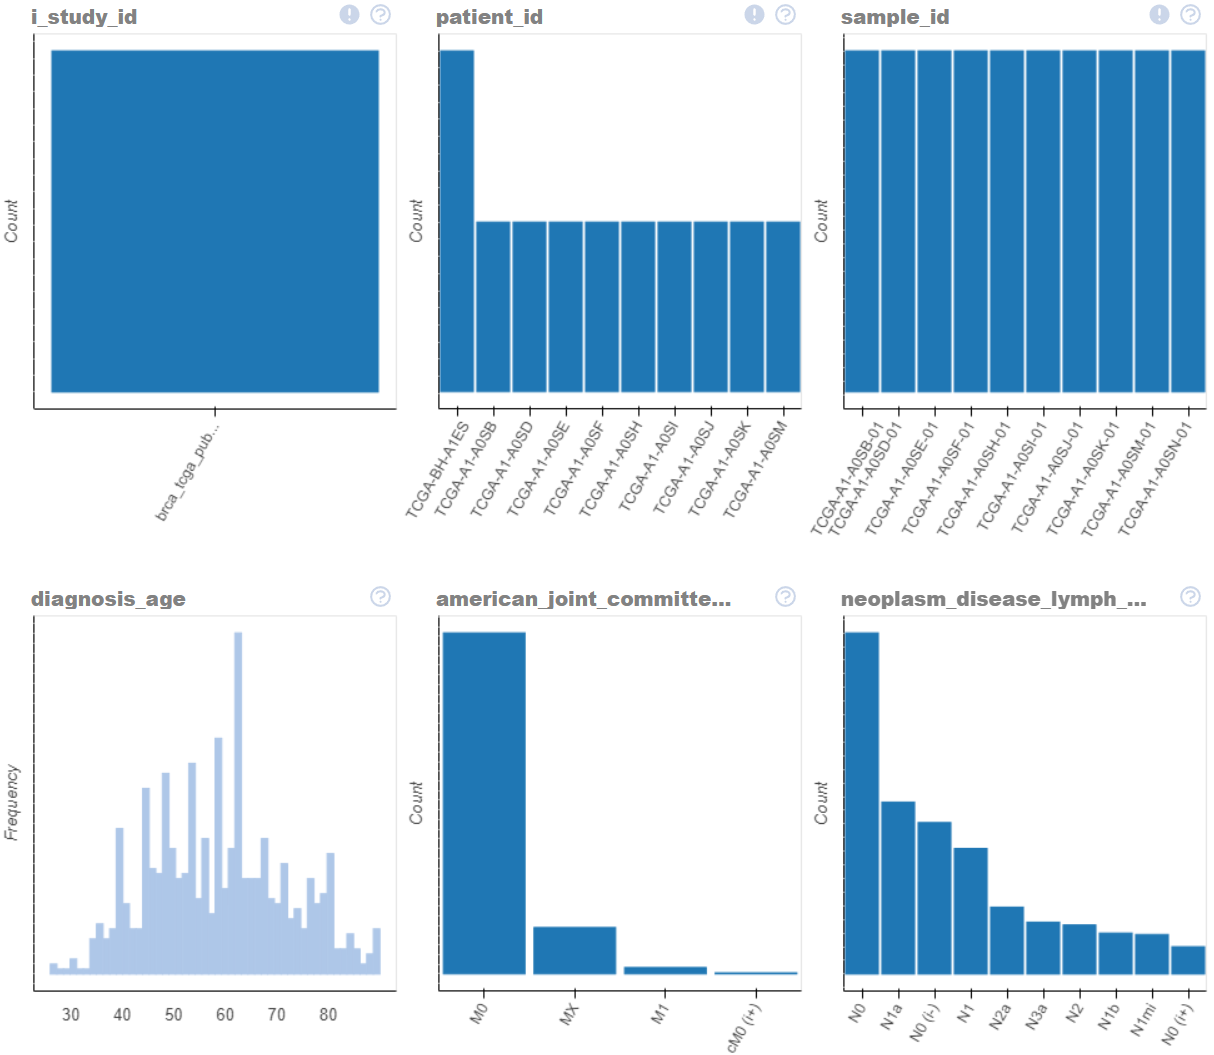
\includegraphics[width=1
	\linewidth]{NOTEBOOK/IMAGES_EDA/1}
\end{figure}

\begin{figure}
	\centering
	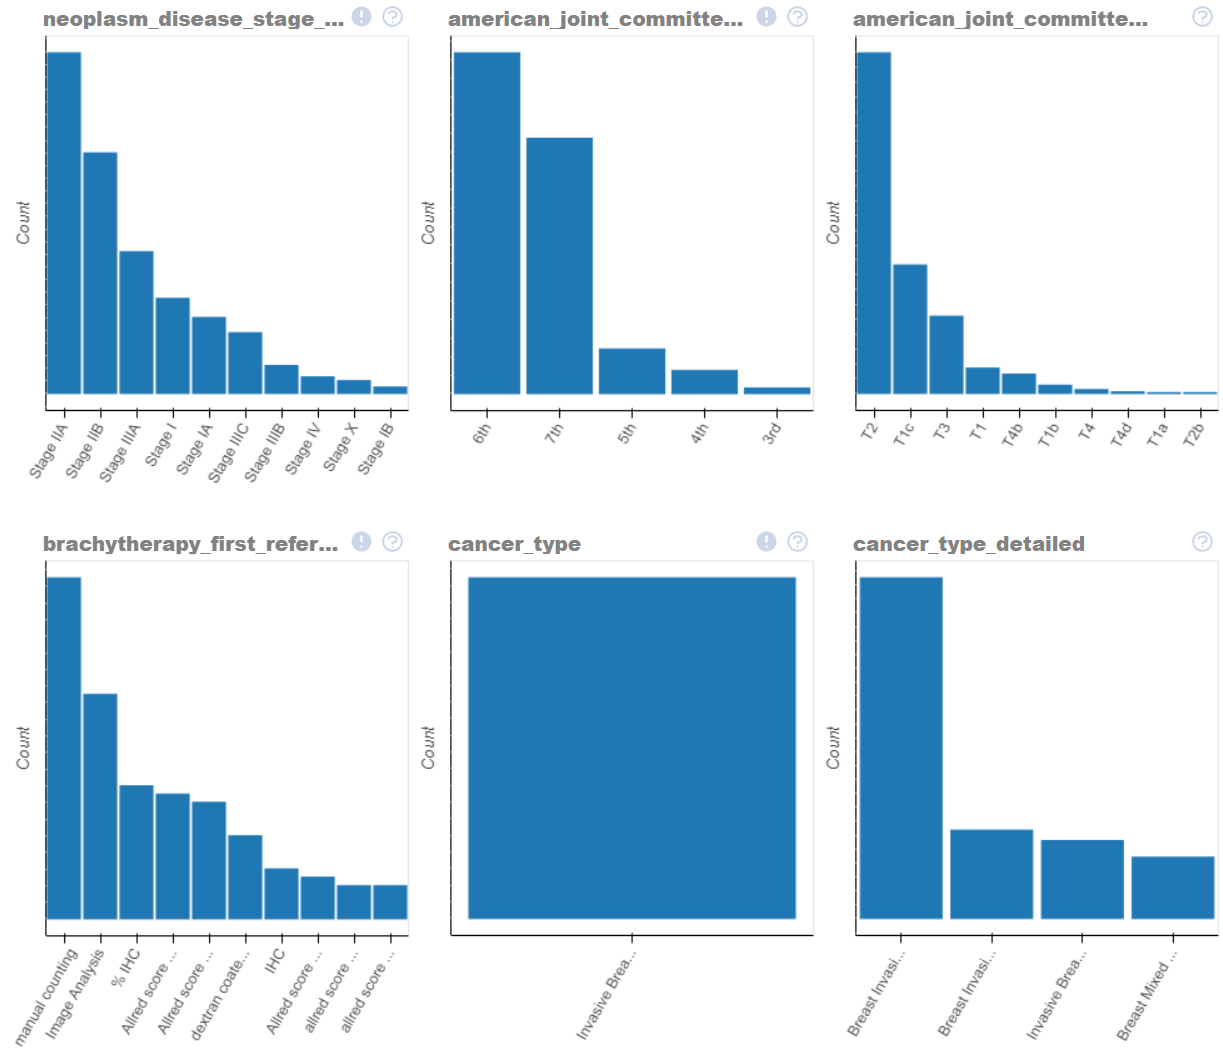
\includegraphics[width=1
	\linewidth]{NOTEBOOK/IMAGES_EDA/2}
\end{figure}

\begin{figure}
	\centering
	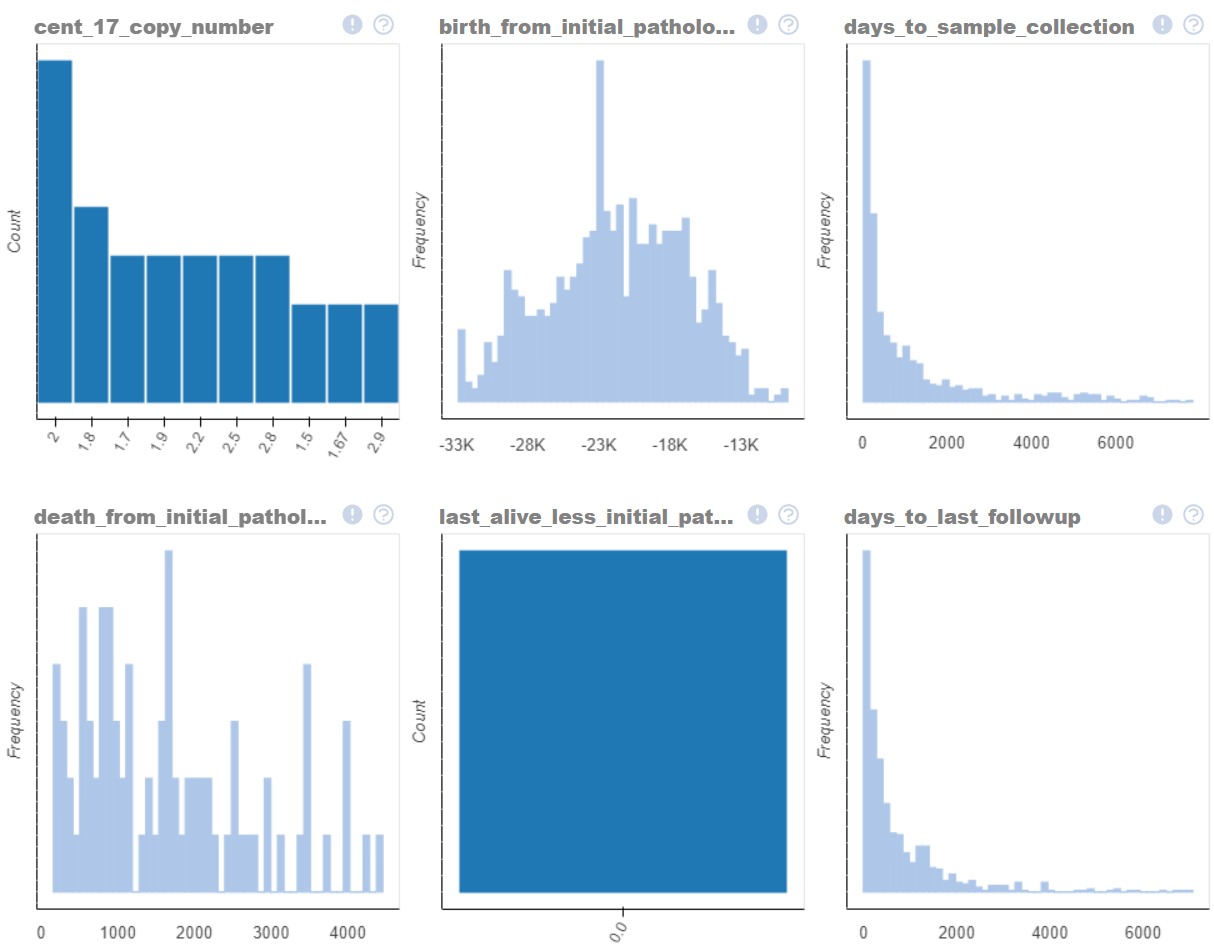
\includegraphics[width=1
	\linewidth]{NOTEBOOK/IMAGES_EDA/3}
\end{figure}

\begin{figure}
	\centering
	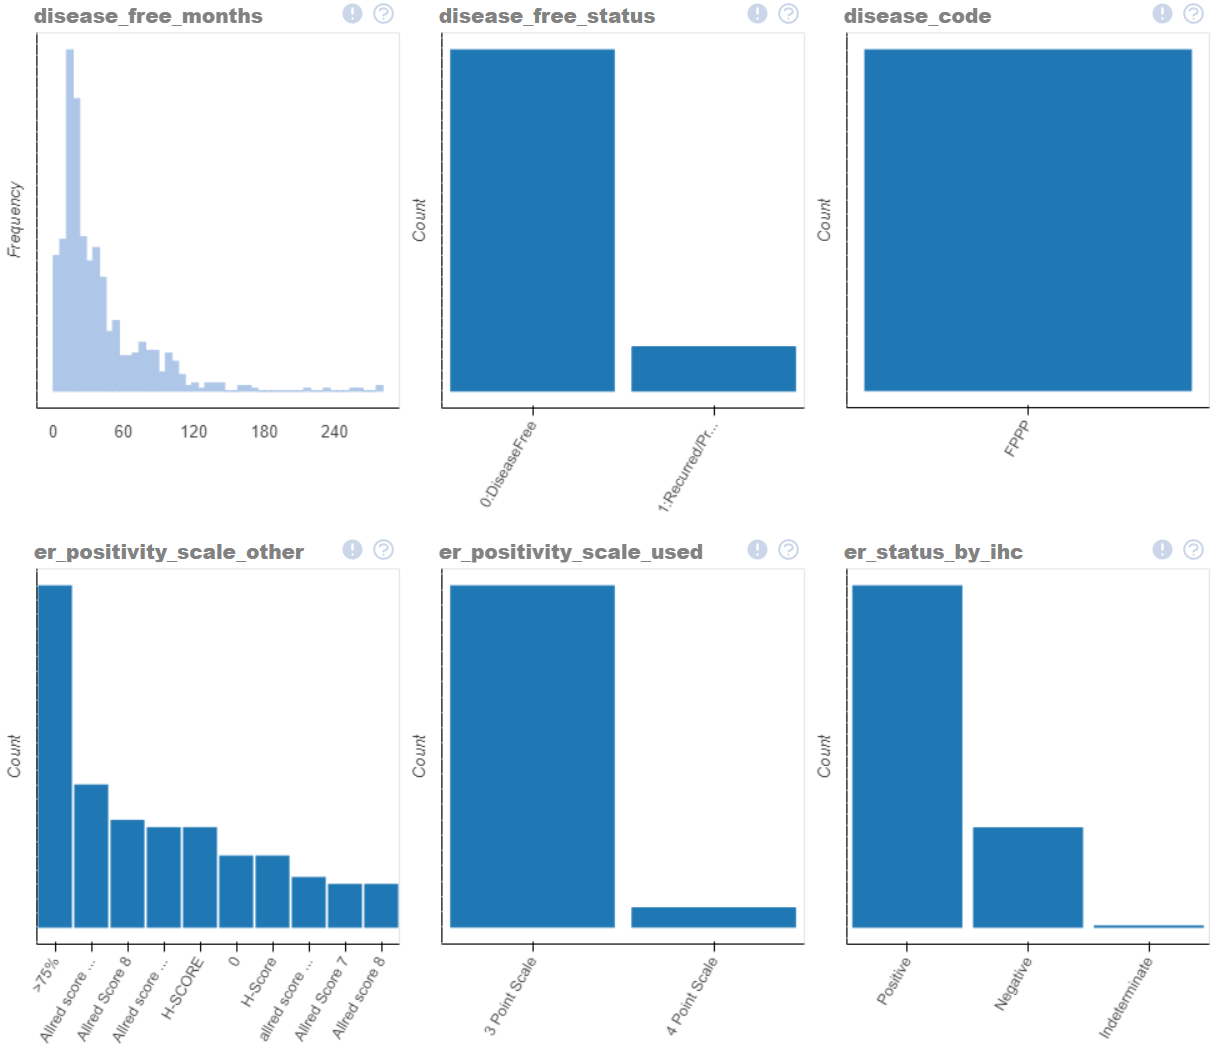
\includegraphics[width=1
	\linewidth]{NOTEBOOK/IMAGES_EDA/4}
\end{figure}

\begin{figure}
	\centering
	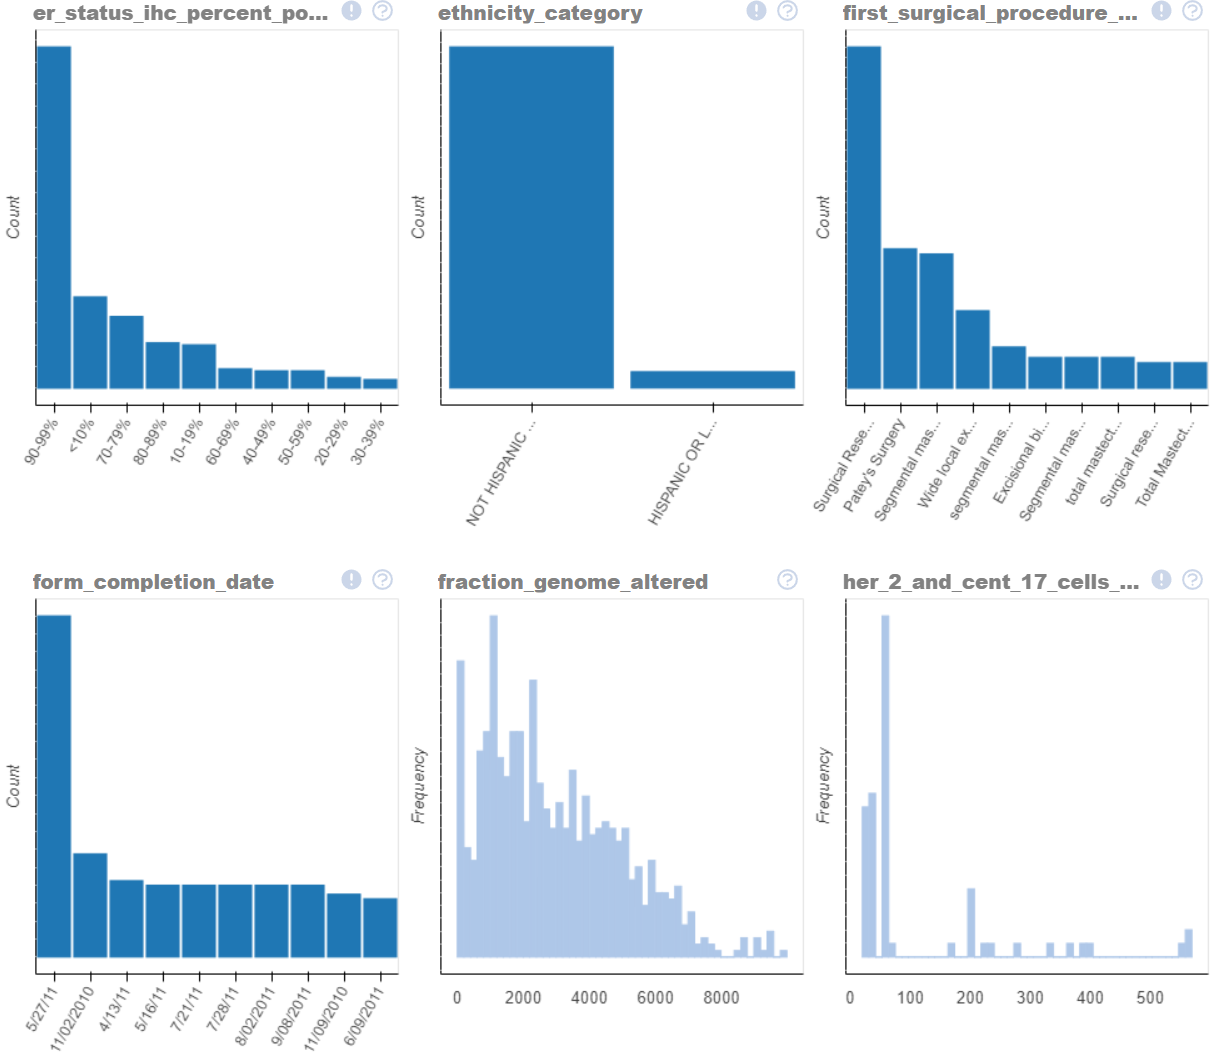
\includegraphics[width=1
	\linewidth]{NOTEBOOK/IMAGES_EDA/5}
	\label{EDA}
	\caption{Distribución del conjunto de datos del Carcinoma invasivo de mama.}\label{fig:foobar}
\end{figure}


\subsection{Detección de datos Ausentes}
En segundo lugar, basados en la obtención de los atributos del conjunto de datos \textit{“Breast Invasive Carcinoma (TCGA, Cell 2015)”}, se realizo un análisis de la cantidad de datos perdidos para identificar las variables y en la etapa posterior realizar la limpieza y el pre-procesamiento de los datos de destino hacerlos consistentes y sin ningún tipo de ruido. Los resultados obtenidos se pueden observar en la figura \ref{Missing_Bar_Chart}:


\begin{figure}[!htb]
	\centering
	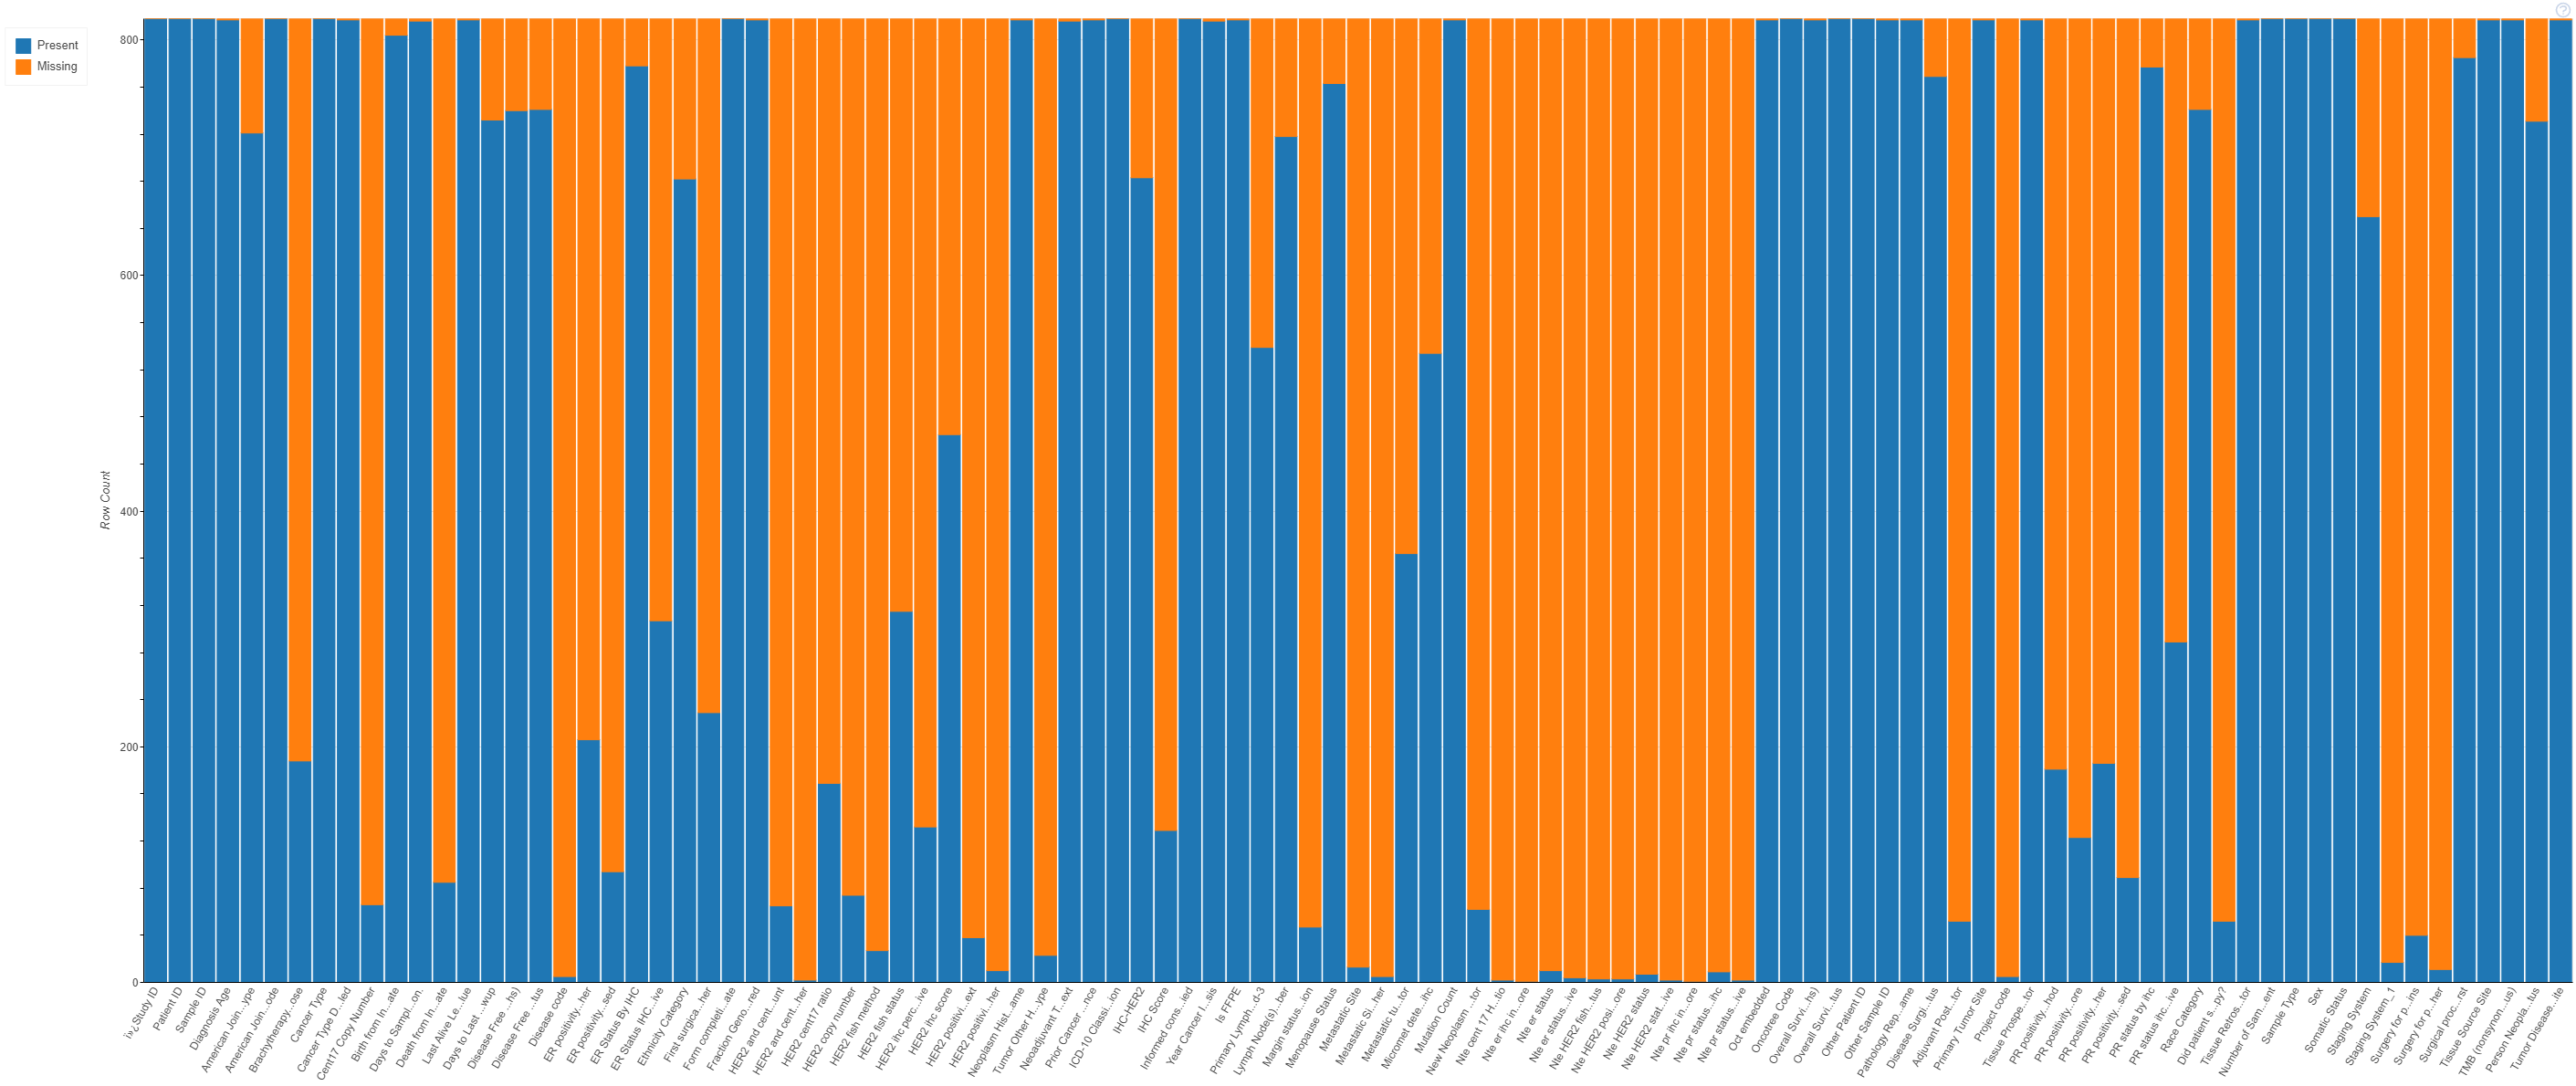
\includegraphics[width=1\linewidth]{IMAGENES/Missing_Bar_Chart}
	\caption{Datos perdidos expresados en una gráfica de barras.}
	\label{Missing_Bar_Chart}
\end{figure}

\begin{figure}[!htb]
	\centering
	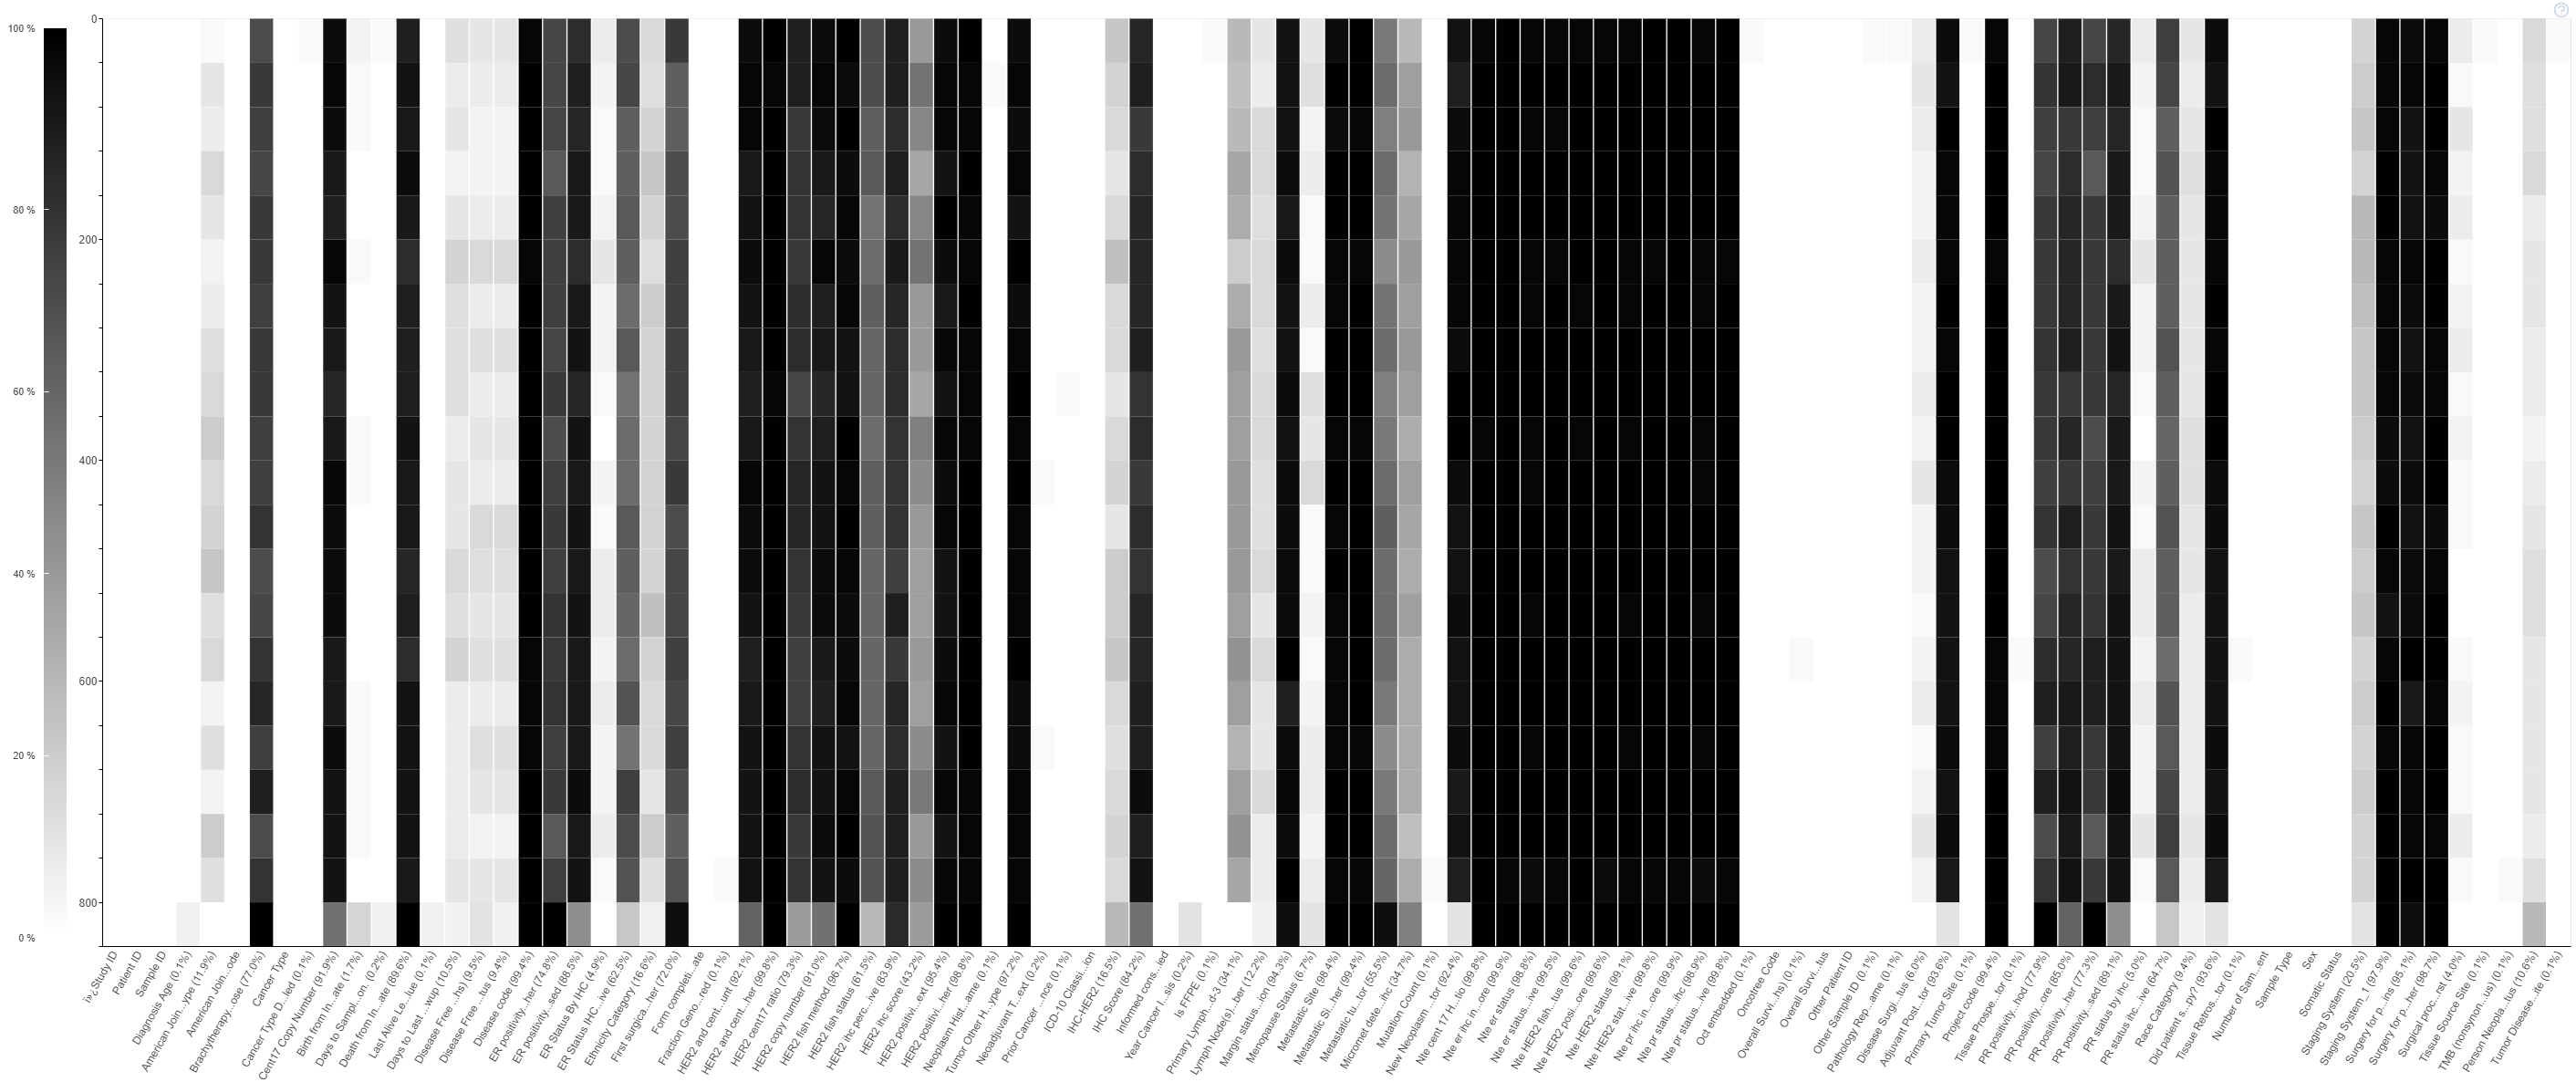
\includegraphics[width=1
	\linewidth]{IMAGENES/Missing_Spectrum}
	\caption{Datos perdidos expresados en un diagrama espectral.}
	\label{Missing_Spectrum}
\end{figure}


\subsection{Análisis Descriptivo }
En primer lugar, se realizo el respectivo análisis descriptivo para detectar cual es comportamiento de los atributos del conjunto de datos \textit{“Breast Invasive Carcinoma (TCGA, Cell 2015)”}. En la gráfica \ref{EDA} se puede observar las gráficas estadísticas unidimensionales de la 110 variables, las cuales permitieron extraer  las características mas representativas y permitieron identificar el comportamiento de los datos.

\begin{table*}[!htb]
	\footnotesize
	\begin{threeparttable}
		\caption{Conjunto de datos del Carcinoma invasivo de mama (TCGA, Cell 2015).}
		\label{Analisis_Descriptivo}
		\begin{tabular}{p{2.5cm} p{7cm} p{6.5cm}} \toprule
			\begin{center}Variable\end{center}   	 
			&\begin{center}Análisis descriptivo\end{center}             
			&\begin{center}Gráfico estadístico\end{center}\\ \hline
			%------------------------------------------------------	
			Diagnosis Age
			& La \textit{edad de diagnostico} del cáncer de mama tiene una tendencia central de 59 años, en donde la edad mínima presentada es de  26 años y la edad máxima presentada es de 90 años.
			
			& \begin{center}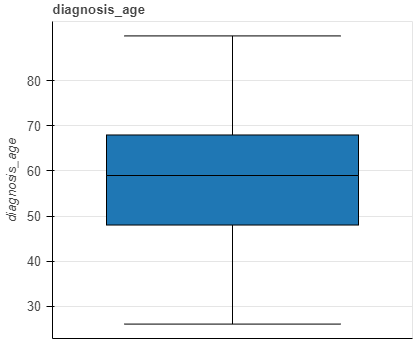
\includegraphics[width=1\linewidth]{NOTEBOOK/IMAGENES_DESCRIPTIVAS/1_diagnosis_age}\end{center}
			\\ \hline
			%------------------------------------------------------	
			AJCC Metastasis Stage Code 
			& El código AJCC para la \textit{estadificación metastásica(M) del cáncer} se visualiza en orden descendente de la siguiente manera: En primer lugar, el código \textit{m0} se presenta en 707 pacientes en donde el cáncer hizo metástasis pero no se  disemino a otras partes del cuerpo. En segundo lugar se encuentra el código \textit{mx} presentado en 96 pacientes a los cuales no fue posible medir la metástasis. En tercer lugar se encuentra el código \textit{m1} presentado en 13 pacientes en donde el cáncer se diseminó a otras partes del cuerpo. En ultimo lugar se encuentra el código \textit{cM0(i+)} presentado en 2 pacientes en los cuales no se detecto evidencia de metástasis a distancia, pero hubo un pequeño número de células en las cuales se encontró una metástasis diminuta (no mayor de 0.2 mm) detectada en ganglios linfáticos no regionales \cite{NCI}.
			
			& \begin{center}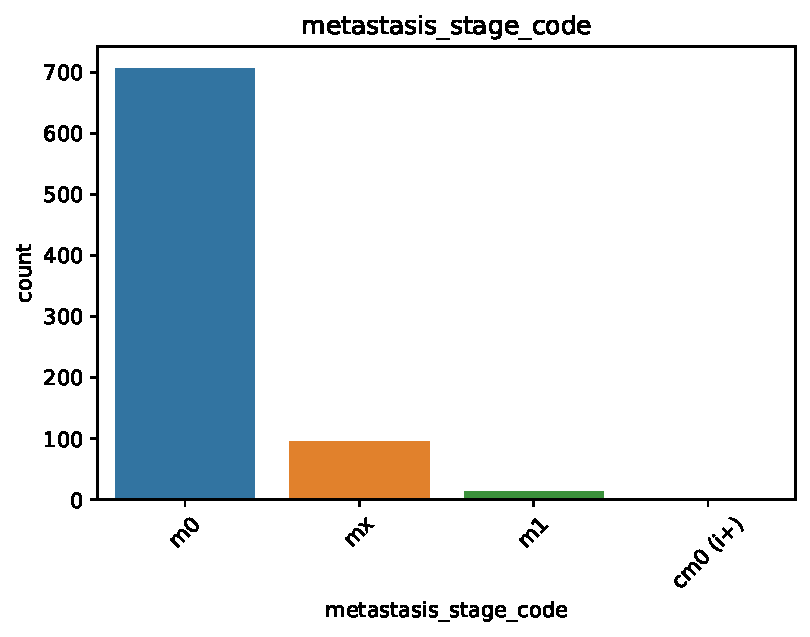
\includegraphics[width=1\linewidth]{NOTEBOOK/IMAGENES_DESCRIPTIVAS/2_metastasis_stage_code}\end{center}
			\\ \hline
			%------------------------------------------------------	
			AJCC Neoplasm Disease Lymph Node Stage Code
			& El código AJCC para la \textit{estadificación del cáncer por neoplasia del ganglio linfático(N)} se visualiza en orden descendente de la siguiente manera: En primer lugar, el código \textit{n0} se presenta en 250 pacientes en donde no hay cáncer en los ganglios linfáticos cercanos. En segundo lugar, el código \textit{n1a} se presento en 126 pacientes en donde el cáncer se diseminó a 1 ganglio linfáticos debajo del brazo con al menos un área de cáncer diseminada de más de 2 mm de ancho. En tercer lugar el código \textit{n0(i-)} se presento en 126 pacientes en donde, no hay evidencia histológica de metástasis en los ganglios linfáticos regionales. Del cuarto lugar en adelante, se refiere a la cantidad y ubicación de los ganglios linfáticos que contienen cáncer. Cuanto mayor sea el número después de la $n$, más ganglios linfáticos se vieron afectados.	
			
			& \begin{center}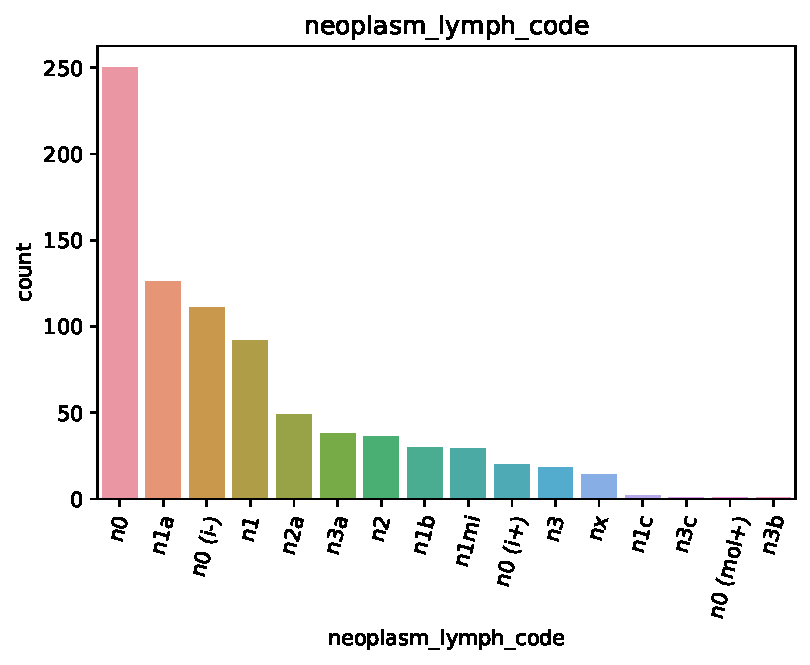
\includegraphics[width=1\linewidth]{NOTEBOOK/IMAGENES_DESCRIPTIVAS/3_neoplasm_lymph_code}\end{center}
			\\ \hline
			%------------------------------------------------------	
		\end{tabular}
	\end{threeparttable}
\end{table*}

\begin{table*}[!htb]
	\footnotesize
	\begin{threeparttable}
		\begin{tabular}{p{2.5cm} p{7cm} p{6.5cm}} \toprule
			%------------------------------------------------------	
			AJCC Neoplasm Disease Stage Code
			& Las etapas AJCC para la \textit{estadificación del cáncer por neoplasia} se visualiza en orden descendente de la siguiente manera: En primer lugar, la \textit{etapa iia} se presenta en 278 pacientes en donde el tumor mide más de 20 mm pero no más de 50 mm y no se ha propagado a los ganglios linfáticos axilares. En segundo lugar, la \textit{etapa iib} se presento en 190 pacientes en donde el tumor mide más de 50 mm pero no se ha propagado a los ganglios linfáticos axilares. En tercer lugar la \textit{etapa iiia} se presento en 112 pacientes en donde el tumor se diseminó de 4 a 9 ganglios linfáticos axilares o los ganglios linfáticos mamarios internos, pero no se ha propagado a otras partes del cuerpo. En cuarto lugar, la \textit{etapa i} se presento en 75 pacientes  en donde el tumor es pequeño, invasivo y no se ha propagado a los ganglios linfáticos. En quinto lugar, la \textit{etapa ia} se presento en 60 pacientes en donde el tumor mide menos de 20 mm  y no se ha propagado a los ganglios linfáticos. Del sexto lugar en adelante, el tumor puede tener cualquier tamaño y se ha propagado a otros órganos, como los huesos, los pulmones, el cerebro, el hígado, los ganglios linfáticos distantes o la pared torácica.
			
			& \begin{center}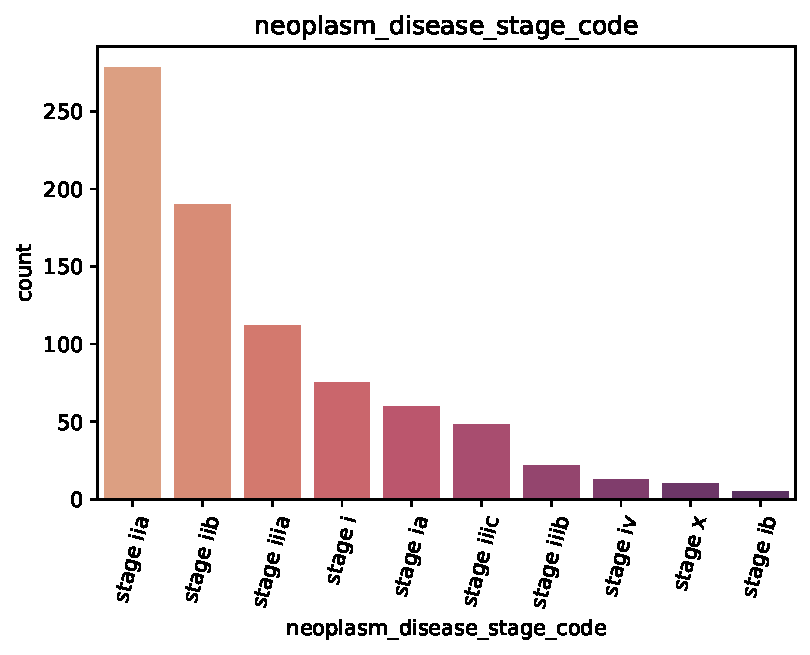
\includegraphics[width=1\linewidth]{NOTEBOOK/IMAGENES_DESCRIPTIVAS/4_neoplasm_disease_stage_code}\end{center}
			\\ \hline
			%------------------------------------------------------	
			AJCC Tumor Stage Code 
			& El código AJCC para la \textit{estadificación el tumor (T) primario del cáncer} se visualiza en orden descendente de la siguiente manera: En primer lugar, el código \textit{t2} se presenta en 459 pacientes en donde el tumor mide más de 20 mm pero no más de 50 mm. En segundo lugar, el código \textit{t1c} se presento en 173 pacientes en donde el tumor mide  de 10 mm a 20 mm o menos. En tercer lugar el código \textit{t3} se presento en 104 pacientes en donde el tumor mide más de 50 mm. En cuarto lugar el código \textit{t1} se presento en 34 pacientes en donde el tumor  mide 20 mm o menos en su área más ancha. En quinto lugar el código \textit{t4b} se presento en 26 pacientes en donde el tumor ha crecido dentro de la piel. Del sexto lugar en adelante, el código \textit{t1b} se presento en 11 pacientes en donde el tumor mide más de 5 mm pero menos de 10 mm, el código \textit{t4} se presento en 5 pacientes en donde el tumor ha crecido hacia la pared torácica, el código \textit{t4d} se presento en 2 pacientes en donde es cáncer de mama inflamatorio, el código \textit{t1a} se presento en 1 paciente en donde el tumor mide más de 1 mm pero menos de 5 mm, el código \textit{t2b} se presento en 1 paciente en donde el tumor mide más de el tumor mide más de 25 mm pero menos de 50 mm.
			
			& \begin{center}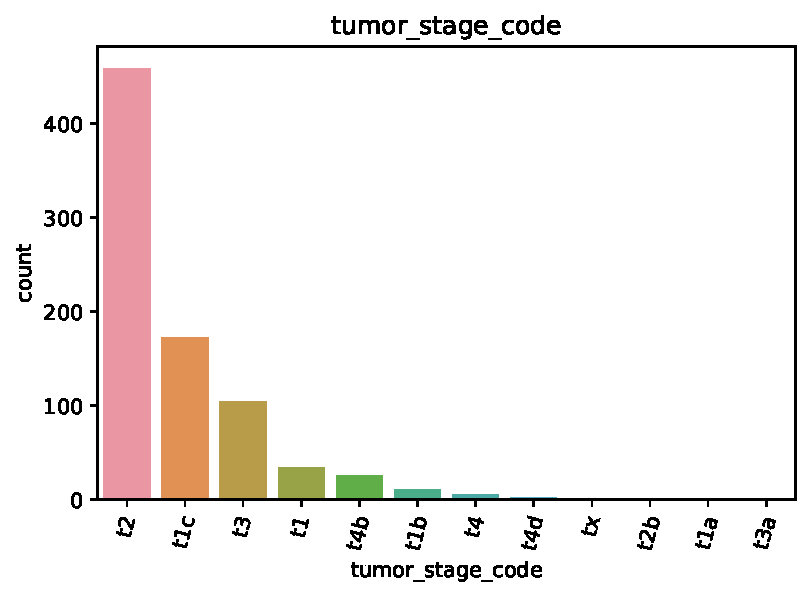
\includegraphics[width=1\linewidth]{NOTEBOOK/IMAGENES_DESCRIPTIVAS/5_tumor_stage_code}\end{center}
			\\ \hline
		\end{tabular}
	\end{threeparttable}
\end{table*}


\begin{table*}[!htb]
	\footnotesize
	\begin{threeparttable}
		\begin{tabular}{p{2.5cm} p{7cm} p{6.5cm}} \toprule
			%------------------------------------------------------	
			Cancer Type Detailed
			& El \textit{tipo de cáncer de mama} se visualiza en orden descendente de la siguiente manera: En primer lugar, el \textit{cáncer Ductal invasivo} se presento en 491 pacientes. En segundo  lugar, el \textit{cáncer Lobulillar invasivo} se presento en 127 pacientes. En tercer lugar, el \textit{cáncer invasivo con otros diagnósticos} se presento en 112 pacientes. En cuarto lugar,  el \textit{cáncer mixto (Ductal y Lobulillar)} se presento en 88 pacientes.
			
			& \begin{center}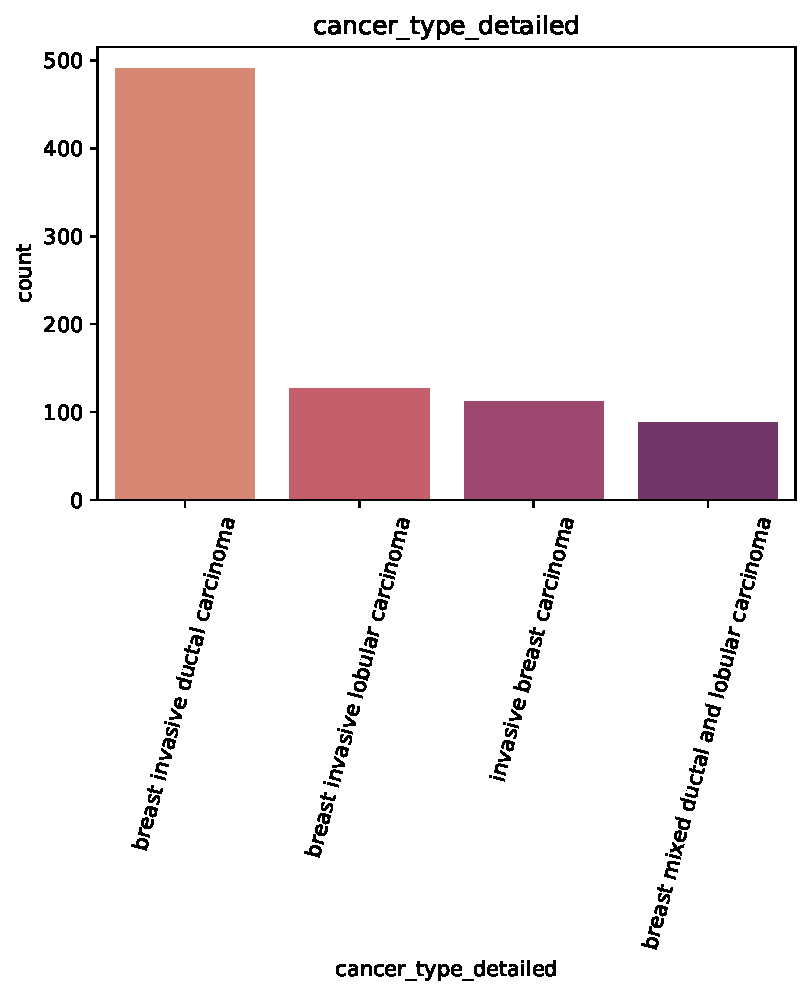
\includegraphics[width=1\linewidth]{NOTEBOOK/IMAGENES_DESCRIPTIVAS/6_cancer_type_detailed}\end{center}
			\\ \hline
			%------------------------------------------------------	
			Days to Sample Collection
			& El intervalo de días para la \textit{recolección de muestras} tiene una tendencia central aproximada de 451 días, en donde el tiempo mínimo presentado es de 16 días y el tiempo máximo presentado de 7804 días.
			
			& \begin{center}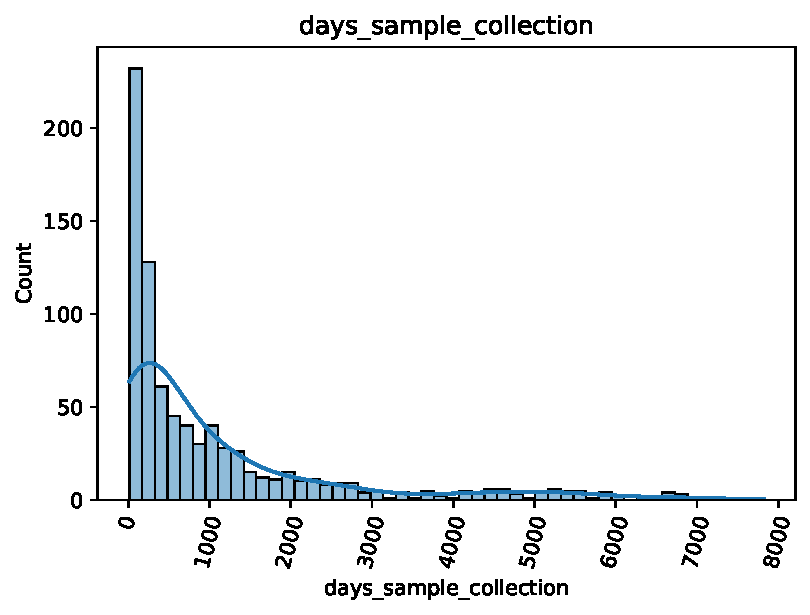
\includegraphics[width=1\linewidth]{NOTEBOOK/IMAGENES_DESCRIPTIVAS/7_days_sample_collection}\end{center}
			\\ \hline
			%------------------------------------------------------	
			Days to Last Followup
			& El Intervalo de tiempo desde la fecha del \textit{último seguimiento} hasta la fecha del diagnóstico patológico inicial tiene una tendencia central aproximada de 579 días, en donde el tiempo mínimo de diagnostico  presentado es de 1 día y el tiempo maximo de diagnostico presentado de 7067 días.
			
			& \begin{center}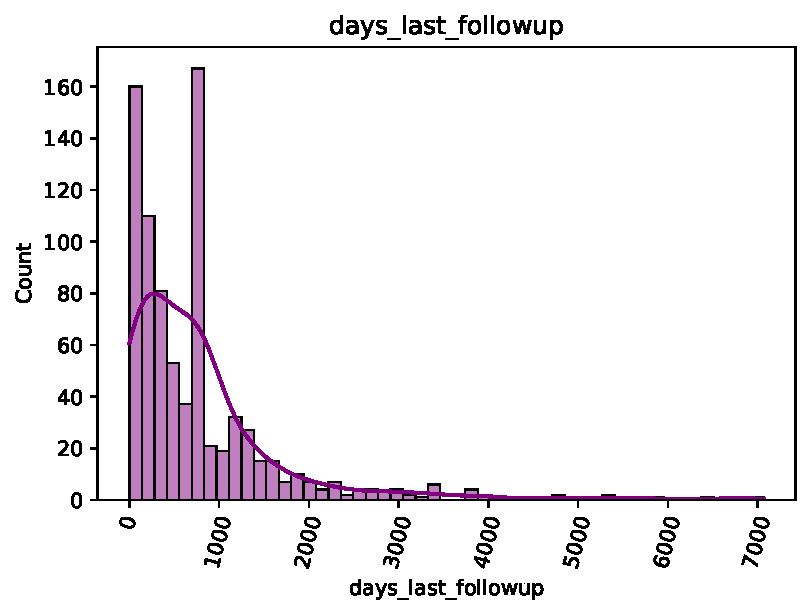
\includegraphics[width=1\linewidth]{NOTEBOOK/IMAGENES_DESCRIPTIVAS/8_days_last_followup}\end{center}
			\\ \hline
		\end{tabular}
	\end{threeparttable}
\end{table*}


\begin{table*}[!htb]
	\footnotesize
	\begin{threeparttable}
		\begin{tabular}{p{2.5cm} p{7cm} p{6.5cm}} \toprule
			%------------------------------------------------------	
			Disease Free (Months)
			& El Intervalo de \textit{meses sin enfermedad} tiene una tendencia central aproximada de 32 meses, en donde el tiempo mínimo presentado es de 16 meses y el tiempo máximo presentado de 281 meses.
			
			& \begin{center}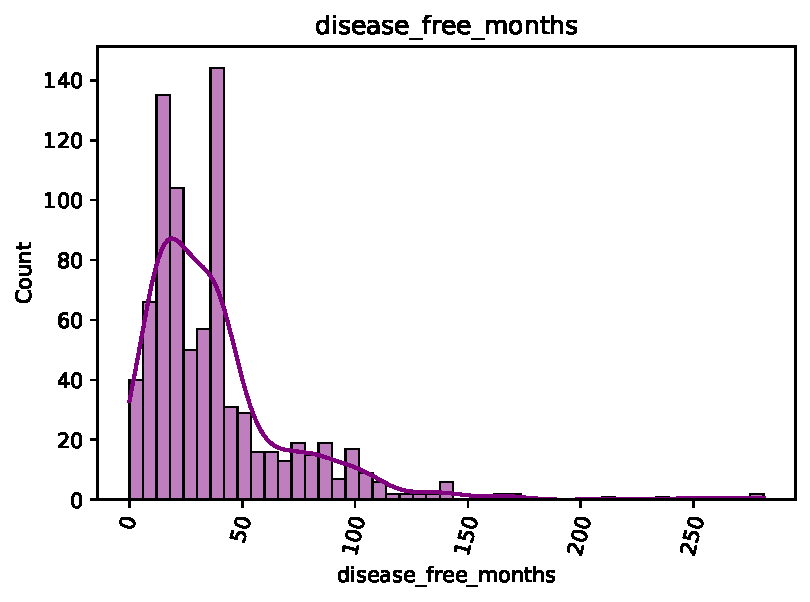
\includegraphics[width=1\linewidth]{NOTEBOOK/IMAGENES_DESCRIPTIVAS/9_disease_free_months}\end{center}
			\\ \hline
			
			%------------------------------------------------------	
			Disease Free Status
			& El \textit{estado libre de enfermedad} se clasifica de forma nominal en dos categorías: La primera categoría corresponde al estado \textit{disease free} en donde se encuentran 733 pacientes que estuvieron libre de enfermedad durante un tiempo determinado y la segunda categoría corresponde al estado el estado \textit{progressed} en donde se encuentran 85 pacientes en donde la enfermedad fue avanzando de manera progresiva. 
			
			& \begin{center}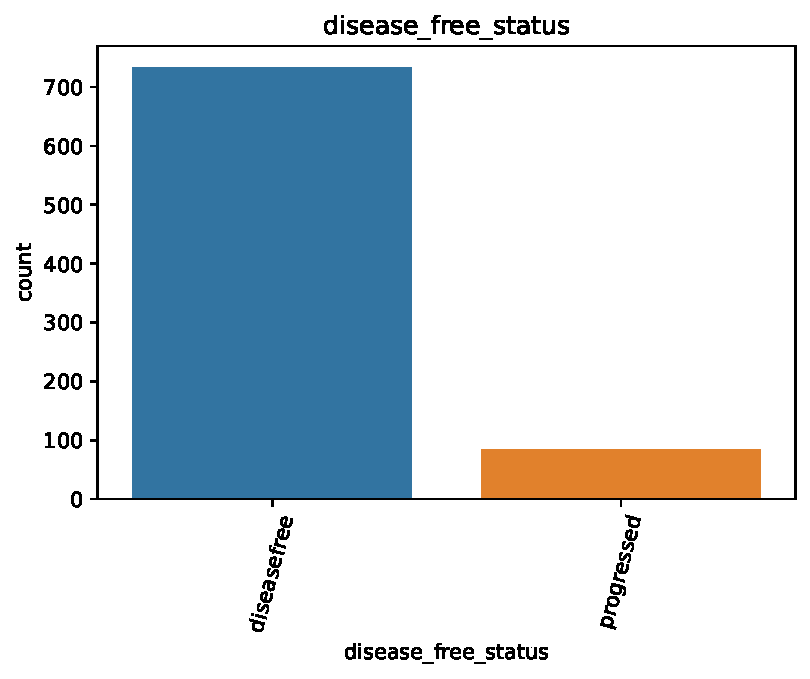
\includegraphics[width=1\linewidth]{NOTEBOOK/IMAGENES_DESCRIPTIVAS/10_disease_free_status}\end{center}
			\\ \hline
			
			%------------------------------------------------------	
			ER positivity scale other
			&La variable \textit{Otra escala de receptor de estrogeno positivo} se visualiza en orden descendente de la siguiente manera: En primer lugar, la escala \textit{allred score 8} se presenta en 671 pacientes que tienen células cancerosas con receptores positivos de estrogeno con un crecimiento fuerte. En segundo lugar, la escala $>$\textit{75\%} se presento en 48 pacientes que tienen células cancerosas con receptores positivos de estrogeno con un crecimiento anormal. En tercer lugar la escala \textit{h-score} se presento en 26 pacientes con un porcentaje moderado de células tumorales con tinción de membrana celular positivo de estrogeno. En cuarto, la escala \textit{allred score 0} se presenta en 15 pacientes que tienen células cancerosas con receptores negativos de estrogeno. Del quinto lugar en adelante, los pacientes presentan células cancerosas con receptores positivos de estrogeno con un comportamiento de crecimiento moderado.
			& \begin{center}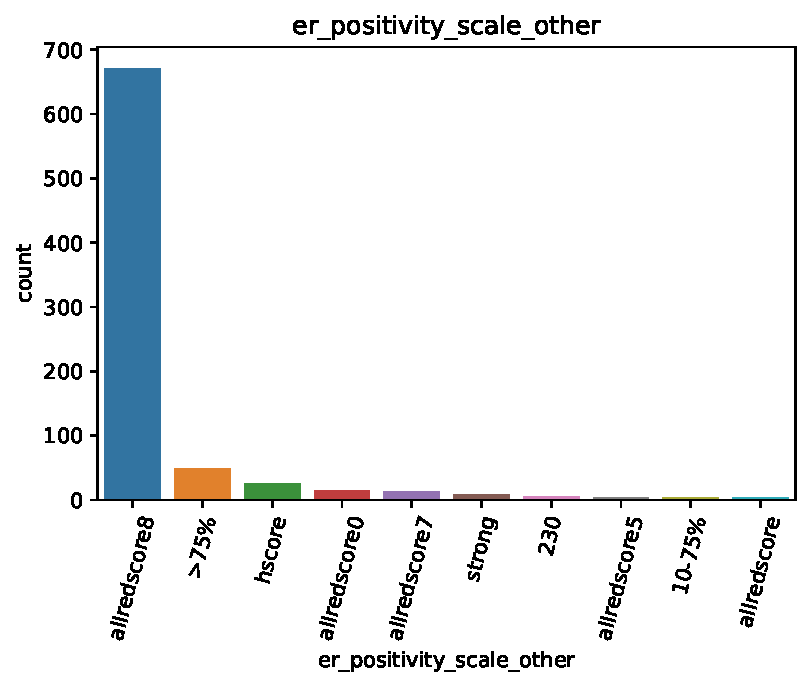
\includegraphics[width=1\linewidth]{NOTEBOOK/IMAGENES_DESCRIPTIVAS/11_er_positivity_scale_other}\end{center}
			\\ \hline
		\end{tabular}
	\end{threeparttable}
\end{table*}

\begin{table*}[!htb]
	\footnotesize
	\begin{threeparttable}
		\begin{tabular}{p{2.5cm} p{7cm} p{6.5cm}} \toprule
			ER Status By IHC
			&El \textit{Estado del receptor de estrogeno por análisis IHC} se clasifica de forma nominal en dos categorías: La primera categoría corresponde al estado \textit{positive} en donde se encuentran 643 pacientes a los cuales al realizar el análisis de inmunohistoquímica(IHC) sobre tejido mamario canceroso se determino que las células cancerosas tienen receptores positivos de estrogeno y la segunda categoría corresponde al estado \textit{negative} en donde se encuentran 175 pacientes a los cuales al realizar el análisis IHC sobre tejido mamario canceroso se determino que las células cancerosas no presentan receptores de estrogeno.
			& \begin{center}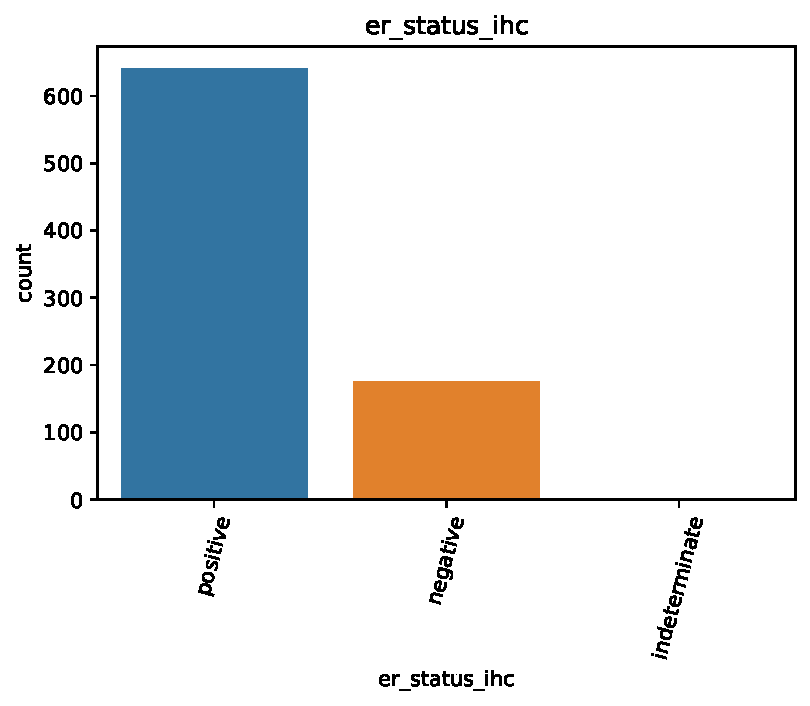
\includegraphics[width=1\linewidth]{NOTEBOOK/IMAGENES_DESCRIPTIVAS/13_er_status_ihc}\end{center}
			\\ \hline
			
			%------------------------------------------------------	
			ER Status IHC Percent Positive
			&El \textit{Estado del porcentaje del receptor de estrogeno por análisis IHC} se visualiza en orden descendente de la siguiente manera: En primer lugar, 668 pacientes presentan células cancerosas con receptores positivos de estrogeno en un \textit{90-99\%} obre tejido mamario. En segundo lugar, 42 pacientes presentan células cancerosas con receptores positivos de estrogeno en un $<$\textit{10\%} sobre tejido mamario. En tercer lugar, 33 pacientes presentan células cancerosas con receptores positivos de estrogeno en un \textit{70-79\%} sobre tejido mamario. En cuarto lugar, 21 pacientes presentan células cancerosas con receptores positivos de estrogeno en un \textit{80-89\%} sobre tejido mamario. En quinto lugar, 20 pacientes presentan células cancerosas con receptores positivos de estrogeno en un \textit{10-19\%} sobre tejido mamario. Del sexto lugar en adelante, los pacientes presentan células cancerosas con receptores positivos de estrogeno con un porcentaje variable.
			& \begin{center}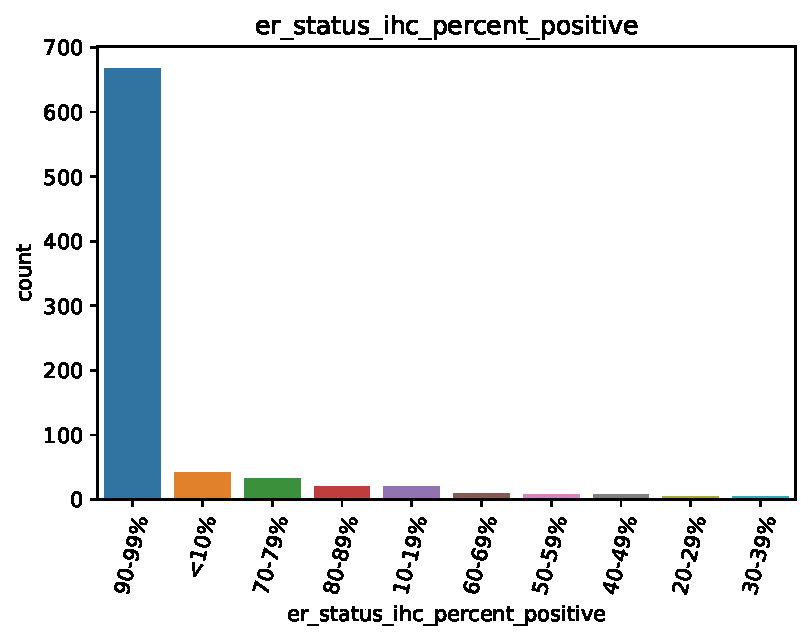
\includegraphics[width=1\linewidth]{NOTEBOOK/IMAGENES_DESCRIPTIVAS/14_er_status_ihc_percent_positive}\end{center}
			\\ \hline
			
			%------------------------------------------------------	
			Ethnicity Category
			&La \textit{Categoría étnica} se clasifica de forma nominal en dos categorías: La primera categoría corresponde al estado \textit{not hispanic or latino} en donde se encuentran 787 pacientes que no presentan una ascendencia latina o de origen español y la segunda categoría corresponde al estado estado \textit{hispanic or latino} en donde se encuentran 31 pacientes que presentan una ascendencia latina o de origen español.
			& \begin{center}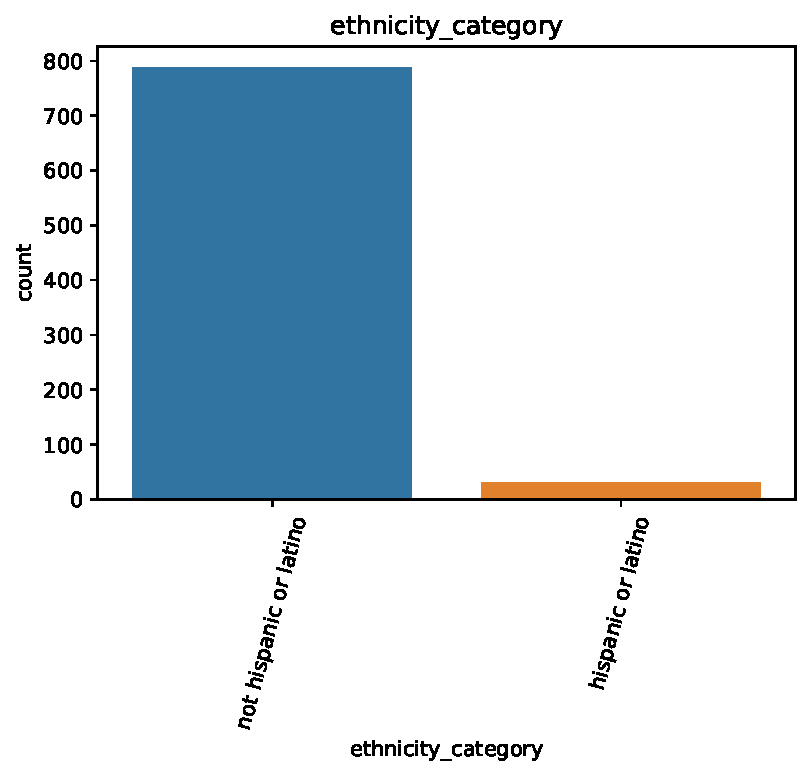
\includegraphics[width=1\linewidth]{NOTEBOOK/IMAGENES_DESCRIPTIVAS/15_ethnicity_category}\end{center}
			\\ \hline
			
		\end{tabular}
	\end{threeparttable}
\end{table*}

\begin{table*}[!htb]
	\footnotesize
	\begin{threeparttable}
		\begin{tabular}{p{2.5cm} p{7cm} p{6.5cm}} \toprule
			%------------------------------------------------------	
			First surgical procedure other
			& La \textit{Primera intervención quirúrgica} se visualiza en orden descendente de la siguiente manera: En primer lugar, la intervención de \textit{resección quirúrgica} se realizo a 660 pacientes a los cuales se les extirpo todo el tumor o la mayor cantidad posible del mismo. En segundo lugar, la intervención quirúrgica \textit{Cirugía de Patey} se realizo a 44 pacientes a los cuales se les extirpo todo el seno, incluida la piel, el tejido mamario, la areola y el pezón junto con la mayoría de los ganglios linfáticos axilares. En tercer lugar, la intervención quirúrgica de \textit{mastectomía segmentaria} se realizo a 34 pacientes a los cuales se les extirpo el cáncer u otro tejido anormal del seno y parte del tejido normal que lo rodea, pero no el seno en sí. En cuarto lugar, la intervención quirúrgica de \textit{escisión local amplia} se realizo a 17 pacientes con los cuales se uso un bisturí para extirpar un tumor u otra lesión anormal y parte del tejido normal que lo rodeaba. En quinto lugar, la intervención quirúrgica \textit{biposia exicional} se realizo a 8 pacientes a los cuales se les extirpo una masa completa o área sospechosa. Del sexto lugar en adelante se utilizaron otros tipos de intervenciones quirúrgicas.
			
			& \begin{center}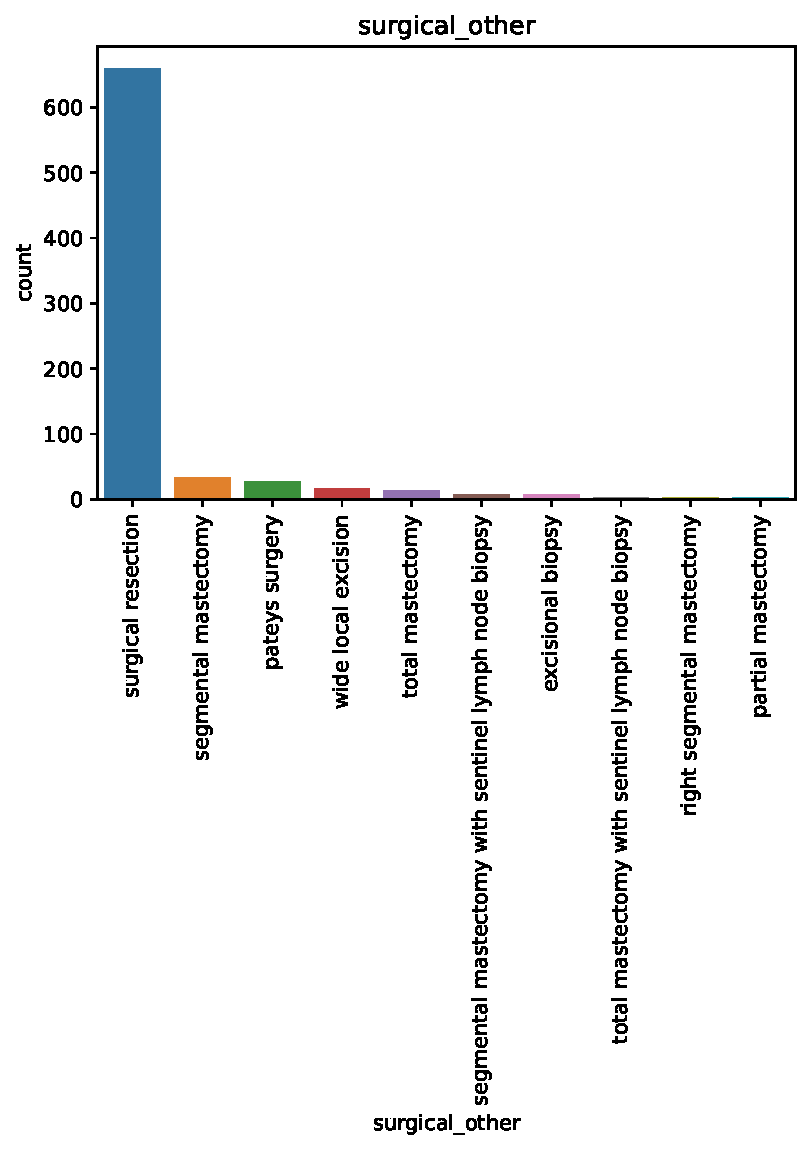
\includegraphics[width=1\linewidth]{NOTEBOOK/IMAGENES_DESCRIPTIVAS/16_surgical_other}\end{center}
			\\ \hline
			
			%------------------------------------------------------	
			Fraction Genome Altered
			& La \textit{Estabilidad genómica} o también llamado \textit{Fenotipo mutador} necesaria para que las células acumulen múltiples mutaciones estimulando el desarrollo del cáncer, presenta un tendencia central de 25.07\% relacionado a genes que se han visto afectados por las ganancias o pérdidas del número de copias celulares, en donde el porcentaje mínimo presentado es del 12,22\% y el máximo del 99,71\%
			
			& \begin{center}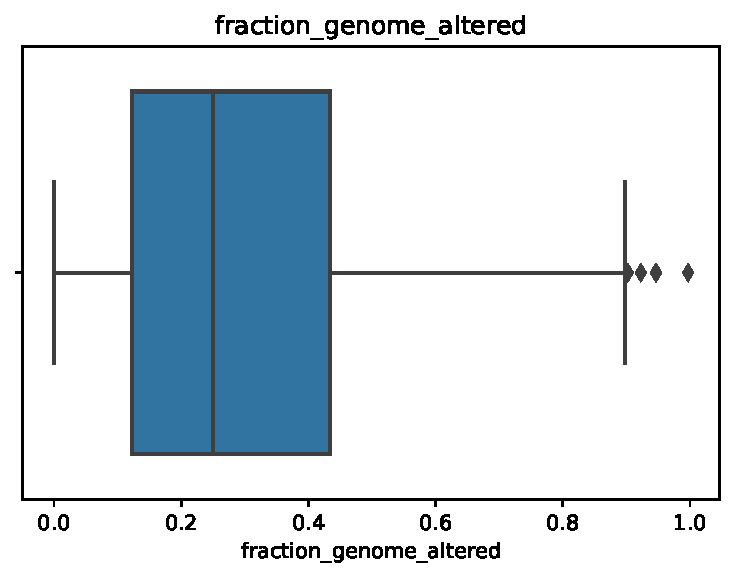
\includegraphics[width=1\linewidth]{NOTEBOOK/IMAGENES_DESCRIPTIVAS/17_fraction_genome_altered}\end{center}
			\\ \hline
			
			%------------------------------------------------------	
			HER2 fish status
			& La \textit{prueba FISH (hibridación fluorescente in situ)} analiza el ADN de las células cancerosas en busca de copias adicionales del gen \textit{HER2 (Receptor 2 del factor de crecimiento epidérmico humano)}. En este caso el \textit{estado FISH} se clasifica de forma nominal en dos categorías: La primera categoría corresponde al estado \textit{negativo} en donde se encuentran 758 pacientes en los cuales la proteína HER2 no está involucrada en el crecimiento del tumor mamario y la segunda categoría corresponde al estado \textit{Positivo} en donde se encuentran 60 pacientes en los cuales las células cancerígenas producen demasiada HER2 estimulando el crecimiento del tumor mamario. 
			& \begin{center}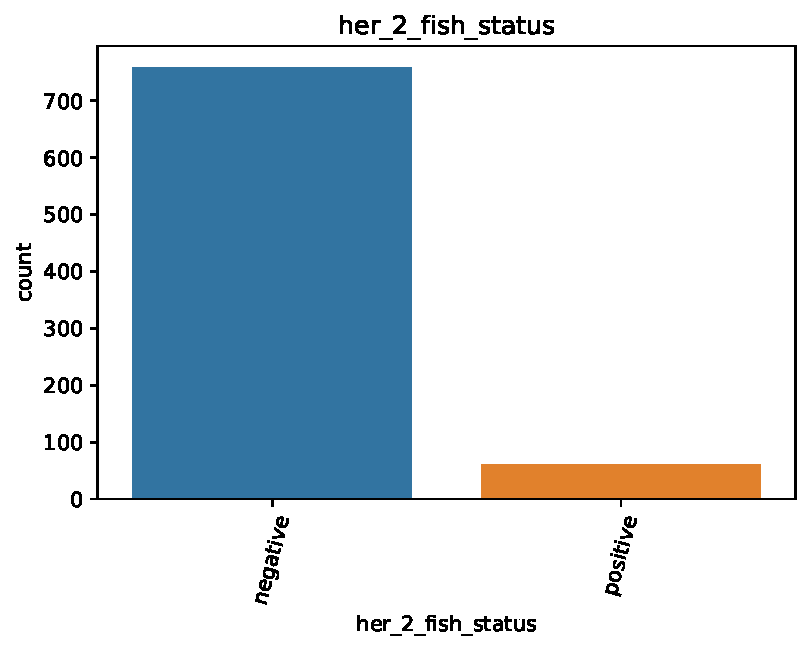
\includegraphics[width=1\linewidth]{NOTEBOOK/IMAGENES_DESCRIPTIVAS/19_her_2_fish_status}\end{center}
			\\ \hline
		\end{tabular}
	\end{threeparttable}
\end{table*}

\begin{table*}[!htb]
	\footnotesize
	\begin{threeparttable}
		\begin{tabular}{p{2.5cm} p{7cm} p{6.5cm}} \toprule
			%------------------------------------------------------	
			HER2 ihc percent positive
			& El \textit{Porcentaje positivo de HER2 según la prueba de inmunohistoquímica (IHC)}, se visualiza en orden descendente de la siguiente manera: En primer lugar, 757 pacientes presentan tinción apenas perceptible, observada en un valor $<$\textit{10\%} de las células tumorales. En segundo lugar, 17 pacientes presentan una tinción de membrana moderada observada en \textit{10-19\%} de las células tumorales. En tercer lugar, 12 pacientes presentan una tinción de membrana intensa observada en \textit{90-99\%} de las células tumorales. Del cuarto lugar en adelante, los pacientes presentan una tinción de membrana variable en un rango de débil a moderada.
			& \begin{center}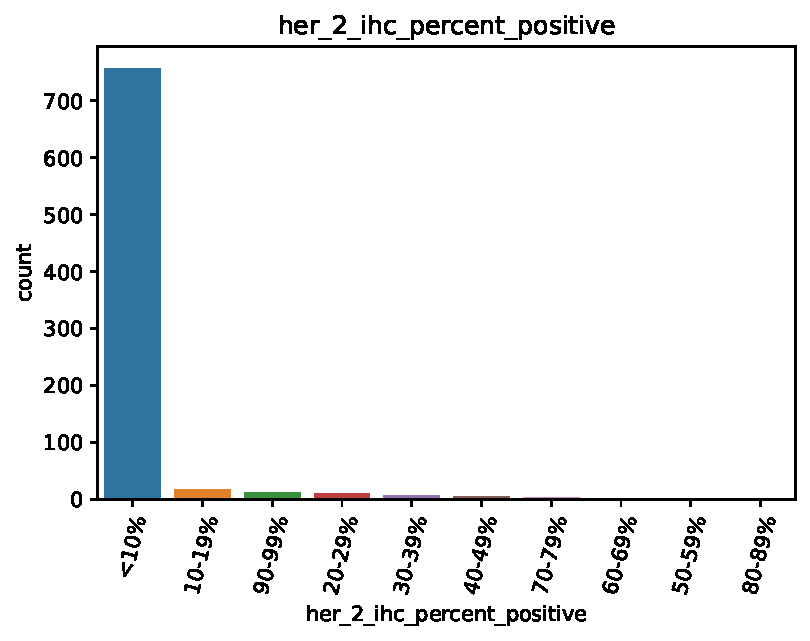
\includegraphics[width=1\linewidth]{NOTEBOOK/IMAGENES_DESCRIPTIVAS/20_her_2_ihc_percent_positive}\end{center}
			\\ \hline
			
			%------------------------------------------------------	
			HER2 ihc score
			& El \textit{puntaje HER2 según la prueba de inmunohistoquímica (IHC)}, se visualiza en orden descendente de la siguiente manera: En primer lugar, 601 pacientes presentan una puntuación \textit{1+}, esto significa  que el tipo de cáncer es HER2-negativo y no es posible tratarlo con medicamentos que tienen a la proteína HER2 como blanco. En segundo lugar, 151 pacientes presentan una puntuación \textit{2+}, esto significa que el estado de HER2 del tumor no está claro, es decir es \textit{ambiguo} y es necesario hacer una prueba del estado FISH para clarificar el resultado. En tercer lugar, 66 pacientes presentan una puntuación \textit{3+}, esto significa que el cáncer es HER2-positivo y es posible tratarlo con medicamentos que tienen a la proteína HER2 como blanco.
			
			& \begin{center}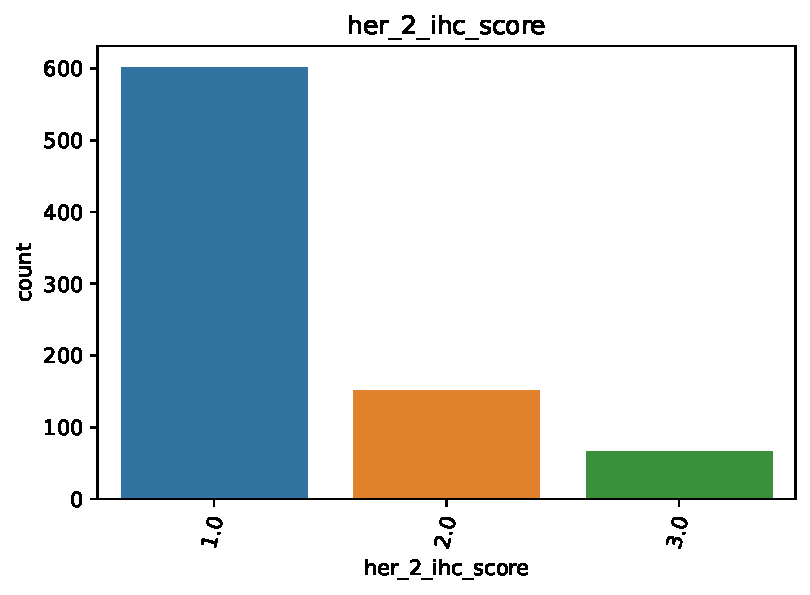
\includegraphics[width=1\linewidth]{NOTEBOOK/IMAGENES_DESCRIPTIVAS/21_her_2_ihc_score}\end{center}
			\\ \hline
			
			%------------------------------------------------------	
			Neoplasm Histologic Type Name
			& El \textit{Nombre del tipo histológico de neoplasia}, se visualiza en orden descendente de la siguiente manera: En primer lugar, 602 pacientes presentan \textit{Carcinoma Ductal Invasivo (IDC)} también llamado \textit{Carcinoma Ductal Infiltrante}. En segundo lugar, 143 pacientes presentan \textit{Carcinoma Lobulillar Invasivo (ILC)} también llamado \textit{Carcinoma Lobulillar Infiltrante.} En tercer lugar, 28 pacientes presentan otro tipo de neoplasia. En cuarto lugar, 23 pacientes presentan \textit{Tumores o Neoplasia mixta (MTCB)}, es decir conformada por los tipos de cáncer LBC e IDC. En quinto lugar, 14 pacientes presentan \textit{Carcinoma Mucinoso (MBC)}. En quinto lugar, 5 pacientes presentan \textit{Carcinoma Medular (MC)}. En sexto lugar, 3 pacientes presentan \textit{Carcinoma Metaplastico (MMC)}.
			& \begin{center}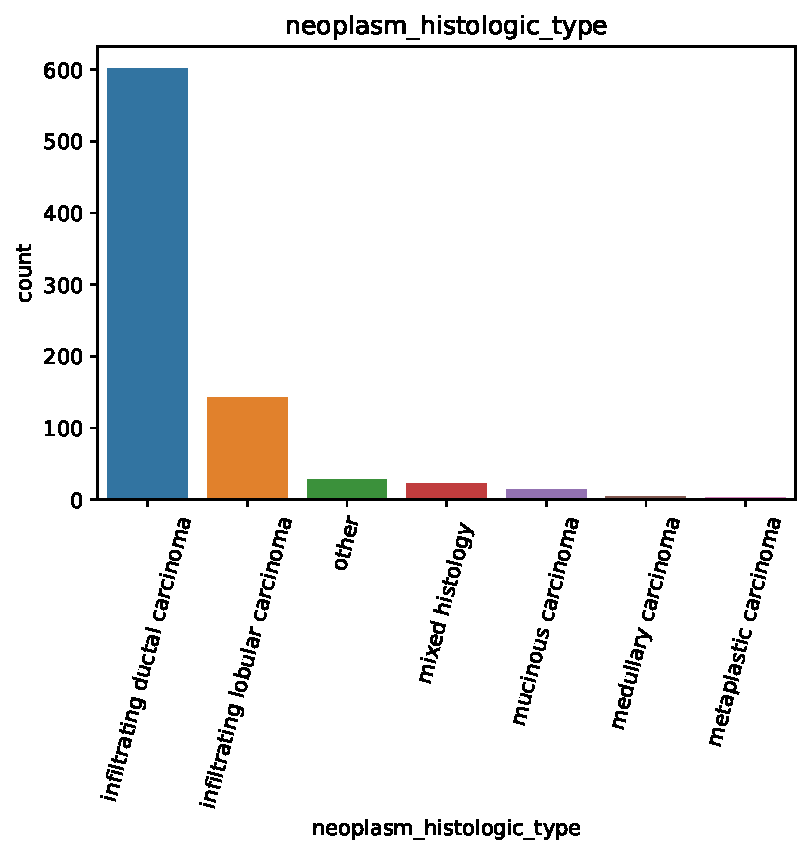
\includegraphics[width=1\linewidth]{NOTEBOOK/IMAGENES_DESCRIPTIVAS/22_neoplasm_histologic_type}\end{center}
			\\ \hline
		\end{tabular}
	\end{threeparttable}
\end{table*}

\begin{table*}[!htb]
	\footnotesize
	\begin{threeparttable}
		\begin{tabular}{p{2.5cm} p{7cm} p{6.5cm}} \toprule
			%------------------------------------------------------	
			Neoadjuvant Therapy Type Administered Prior To Resection Text
			& El \textit{Tratamiento neoadyuvante del paciente} se clasifica de forma nominal en dos categorías: La primera categoría corresponde al estado \textit{No} en donde se encuentran 809 pacientes que no recibieron un tratamiento inicial antes del tratamiento principal y la segunda categoría corresponde al estado \textit{Si} en donde se encuentran 9 pacientes a los cuales se les realizó un tratamiento inicial como quimioterapia, radioterapia o terapia hormonal para reducir el tamaño del tumor antes del tratamiento principal que generalmente consiste en cirugía.
			& \begin{center}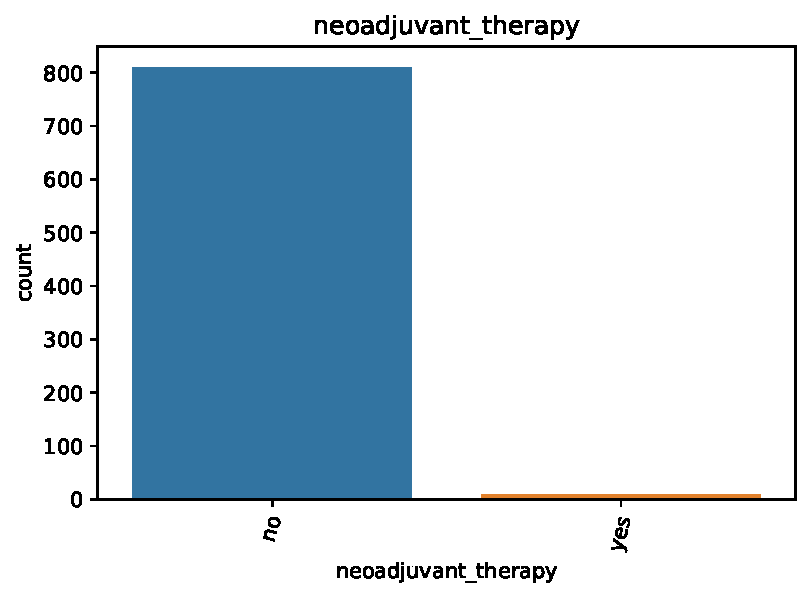
\includegraphics[width=1\linewidth]{NOTEBOOK/IMAGENES_DESCRIPTIVAS/23_neoadjuvant_therapy}\end{center}
			\\ \hline
			
			%------------------------------------------------------	
			ICD-10 Classification
			& El \textit{Diagnóstico de cáncer de mama por medio de la décima revisión ICD} se visualiza en orden descendente de la siguiente manera: En primer lugar, 810 pacientes presentan el código \textit{C50.9} el cual corresponde a una neoplasia maligna de sitio no especificado en la mama derecha. En segundo lugar, 3 pacientes presentan el código \textit{C50.3} el cual corresponde a una neoplasia maligna de cuadrante inferior interno de la mama derecha. En tercer lugar, 2 pacientes presentan el código \textit{C50.4} el cual corresponde a una neoplasia maligna de cuadrante superior externo de la mama derecha. En cuarto lugar, 1 paciente presentan el código \textit{C50.5} el cual corresponde a una neoplasia maligna de cuadrante superior interno de la mama derecha. En quinto lugar, 1 paciente presentan el código \textit{C50.2} el cual corresponde a una neoplasia maligna de cuadrante inferior externo de la mama derecha. En sexto lugar, 1 paciente presentan el código \textit{C50.8} el cual corresponde a una neoplasia maligna de sitios superpuestos de la mama derecha.
			
			& \begin{center}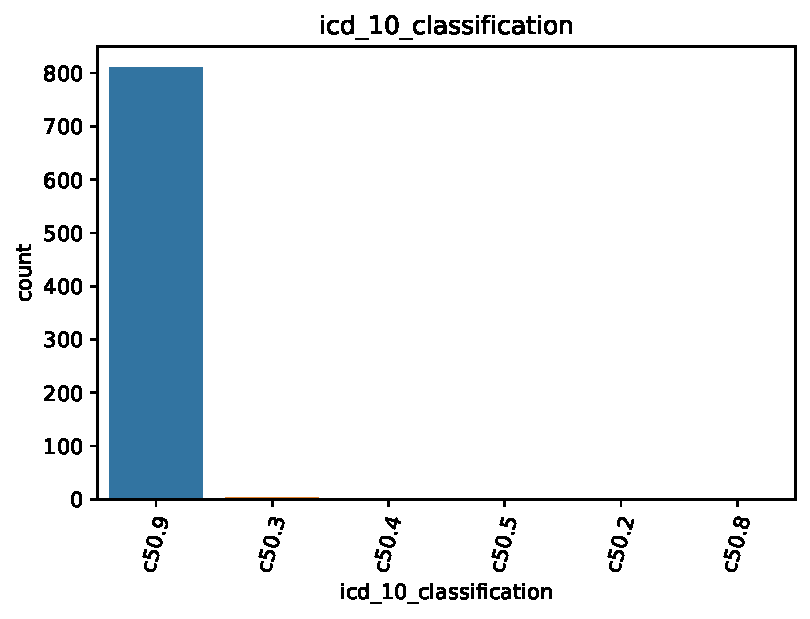
\includegraphics[width=1\linewidth]{NOTEBOOK/IMAGENES_DESCRIPTIVAS/25_icd_10_classification}\end{center}
			
			\begin{center}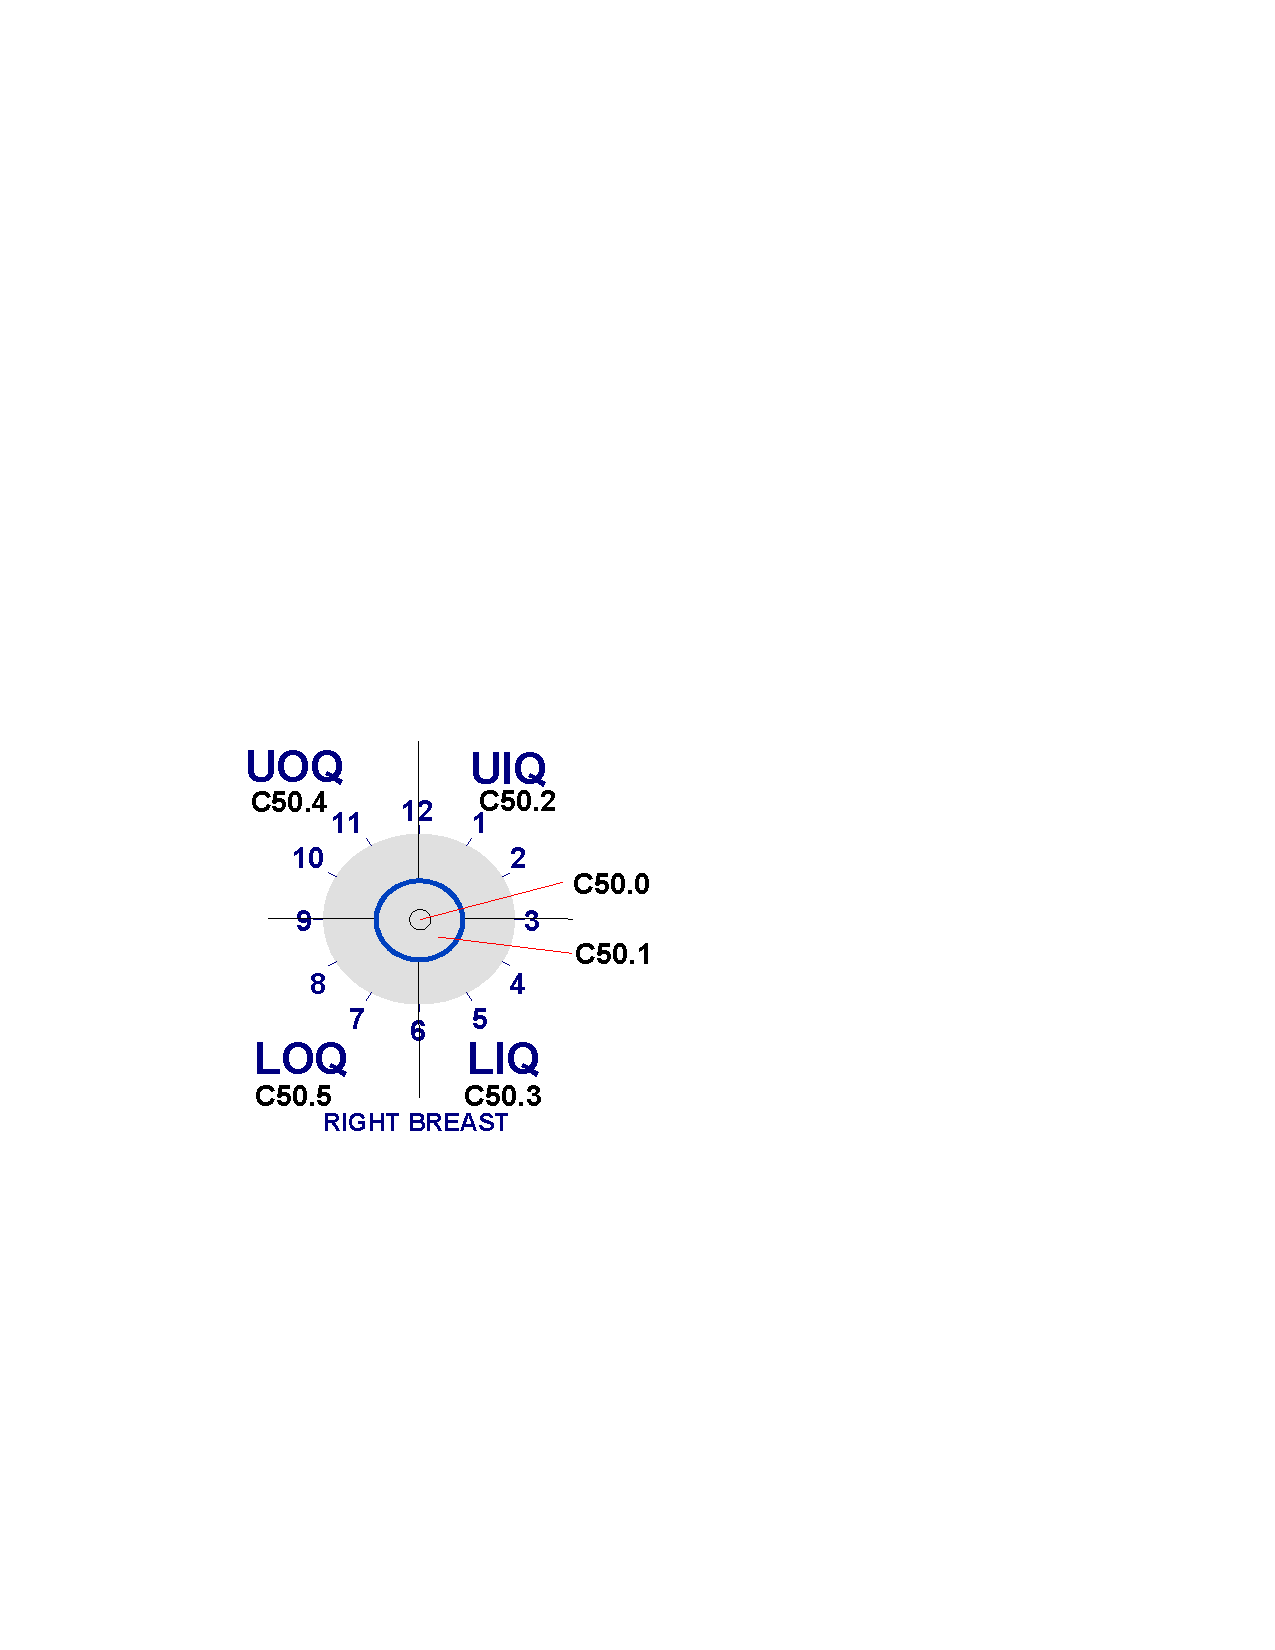
\includegraphics[width=0.75\linewidth]{NOTEBOOK/IMAGENES_DESCRIPTIVAS/25_icd_Breast_Clock_Position}\end{center}
			\\ \hline
			
			%------------------------------------------------------	
			IHC-HER2
			& El \textit{Estado de HER2 según la prueba de inmunohistoquímica (IHC)}, se visualiza en orden descendente de la siguiente manera: En primer lugar, 552 pacientes presentan un estado \textit{negativo}, es decir el cáncer no es posible tratarlo con medicamentos que tienen a la proteína HER2 como blanco. En segundo lugar, 145 pacientes presentan un estado \textit{ambiguo} esto significa que el estado de HER2 del tumor no está claro y es necesario hacer una prueba del estado FISH para clarificar el resultado. En tercer lugar, 121 pacientes presentan un estado \textit{positivo}, es decir el cáncer es posible tratarlo con medicamentos que tienen a la proteína HER2 como blanco.
			& \begin{center}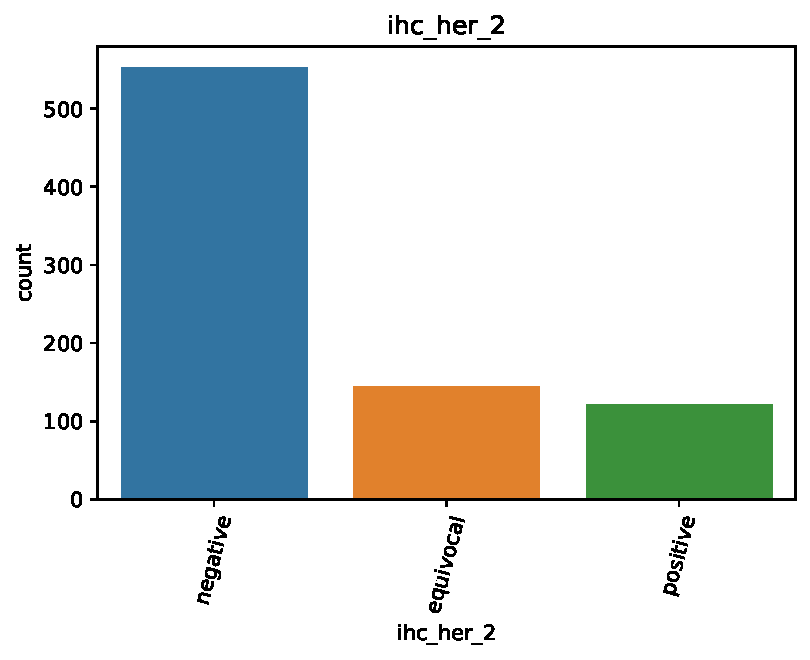
\includegraphics[width=1\linewidth]{NOTEBOOK/IMAGENES_DESCRIPTIVAS/26_ihc_her_2}\end{center}
			\\ \hline
		\end{tabular}
	\end{threeparttable}
\end{table*}

\begin{table*}[!htb]
	\footnotesize
	\begin{threeparttable}
		\begin{tabular}{p{2.5cm} p{7cm} p{6.5cm}} \toprule
			%------------------------------------------------------	
			Year Cancer Initial Diagnosis
			& El intervalo de años para el \textit{Diagnóstico Patológico inicial del cáncer} tiene una tendencia central aproximada en el año 2009, en donde el año de diagnóstico mínimo presentado es 1998 y año de diagnóstico máximo presentado es 2013.
			
			& \begin{center}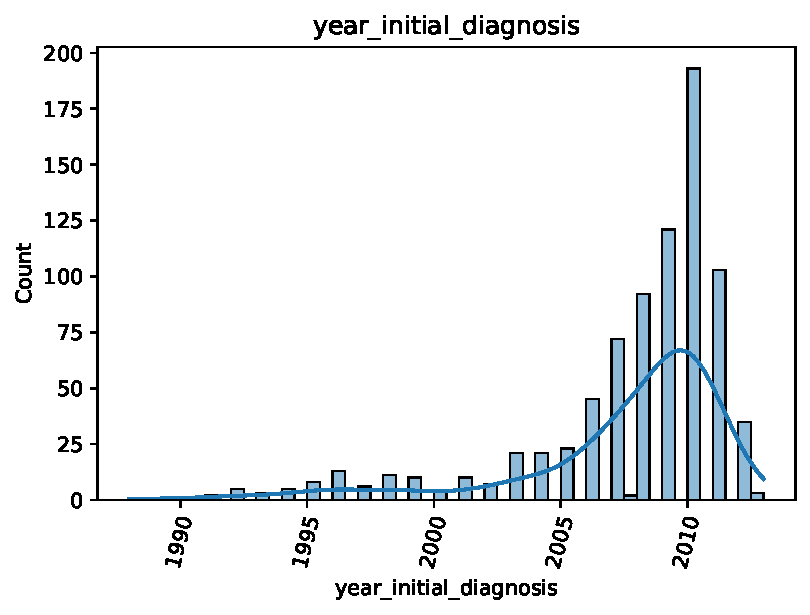
\includegraphics[width=1\linewidth]{NOTEBOOK/IMAGENES_DESCRIPTIVAS/27_year_initial_diagnosis}\end{center}
			\\ \hline
			
			%------------------------------------------------------	
			Primary Lymph Node Presentation Assessment Ind-3
			& La \textit{Evaluación de los ganglios linfáticos} en la presentación primaria de la enfermedad se clasifica de forma nominal en dos categorías: La primera categoría corresponde al estado \textit{Si} en donde se encuentran 798 pacientes en los que el oncólogo detecto la presencia de enfermedad metastásica en los ganglios linfáticos axilares y la segunda categoría al estado \textit{No} en donde se encuentran 20 pacientes en los que el oncólogo no detecto la presencia de enfermedad metastásica.
			
			& \begin{center}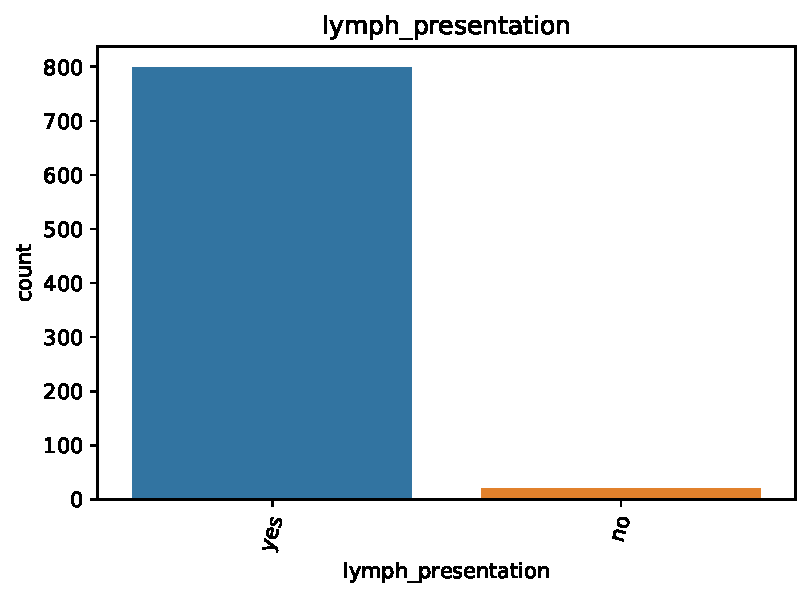
\includegraphics[width=1\linewidth]{NOTEBOOK/IMAGENES_DESCRIPTIVAS/28_lymph_presentation}\end{center}
			\\ \hline
			
			%------------------------------------------------------	
			Positive Finding Lymph Node Hematoxylin and Eosin Staining Microscopy Count
			& El \textit{Recuento de ganglios linfáticos positivos identificados mediante microscopía óptica con tinción de hematoxilina y eosina (H\&E)} tiene una tendencia central aproximada de 5 ganglios linfáticos con estado positivo, es decir que la tinción de hematoxilina presento una mayor proporción evidenciando la presencia de un tumor en crecimiento. Adicionalmente, se puede observar que  el valor mínimo ganglios linfáticos afectados fue 1 y el valor máximo de ganglios linfáticos afectados fue 34. 
			& \begin{center}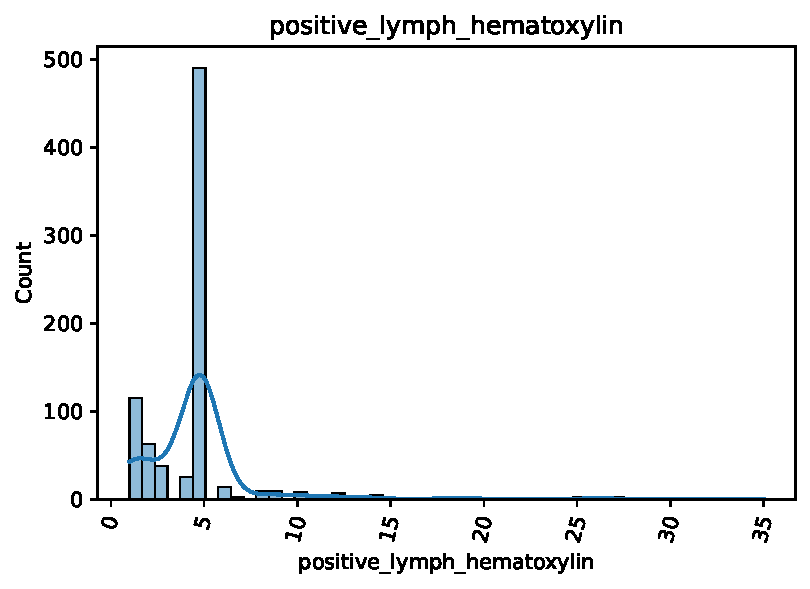
\includegraphics[width=1\linewidth]{NOTEBOOK/IMAGENES_DESCRIPTIVAS/29_positive_lymph_hematoxylin}\end{center}
			\\ \hline
			
			%------------------------------------------------------	
			Lymph Node(s) Examined Number
			& El número de \textit{ganglios linfáticos extirpados} y evaluados patológicamente para la enfermedad tiene una tendencia central aproximada de 10 ganglios linfáticos extirpados , en donde el número mínimo de ganglios linfáticos extirpados es 1 y el número máximo de ganglios linfáticos extirpados es 44.
			& 
			\begin{center}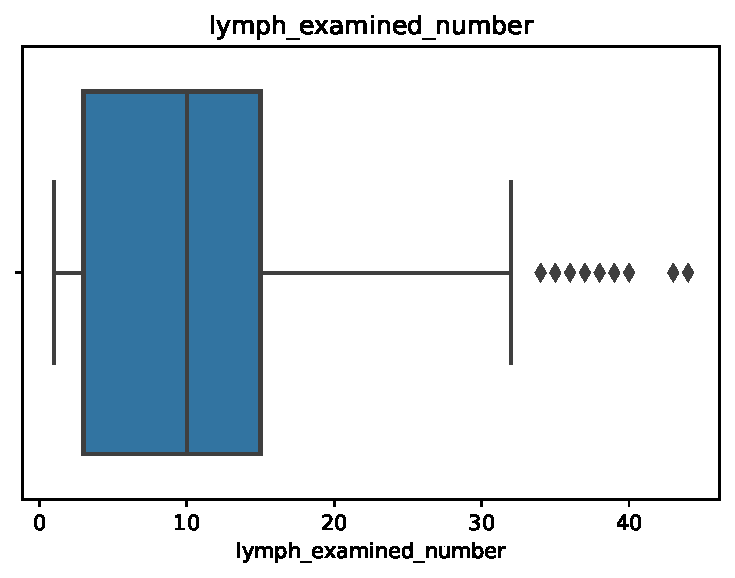
\includegraphics[width=1\linewidth]{NOTEBOOK/IMAGENES_DESCRIPTIVAS/31_lymph_examined_number}\end{center}
			\\ \hline
		\end{tabular}
	\end{threeparttable}
\end{table*}

\begin{table*}[!htb]
	\footnotesize
	\begin{threeparttable}
		\begin{tabular}{p{2.5cm} p{7cm} p{6.5cm}} \toprule
			%------------------------------------------------------	
			Menopause Status
			& El \textit{estado de la menopausia}, se visualiza en orden descendente de la siguiente manera: En primer lugar, 593 pacientes presentan un estado de \textit{PostMenopausia}, en el cual los niveles hormonales permanecen bajos y ya no se presenta un período mensual debido a que los ovarios han dejado de liberar óvulos. En segundo lugar, 166 pacientes presentan un estado de \textit{PreMenopausia}, en el cual la reserva ovárica empieza a disminuir y la mujer pierde su fertilidad. Suele iniciarse sobre los 40 años y tener una duración muy variable, desde pocos años hasta 10 o más. En tercer lugar, 59 pacientes presentan un estado de \textit{PeriMenopausia} el cual se presenta en una etapa más corta que precede a la menopausia y dura hasta los 12 meses posteriores de la última menstruación. Suele durar unos 2 o 3 años y se caracteriza por las irregularidades en el ciclo menstrual. La edad más habitual en la que se presenta la perimenopausia es entre los 45 y los 50 años\cite{ReproAsistidaORG}.
			
			& \begin{center}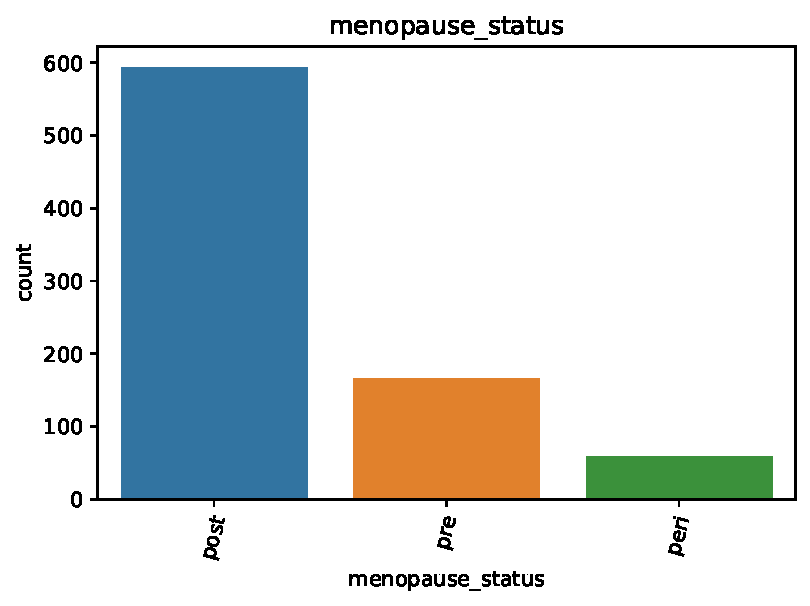
\includegraphics[width=1\linewidth]{NOTEBOOK/IMAGENES_DESCRIPTIVAS/32_menopause_status}\end{center}
			  \begin{center}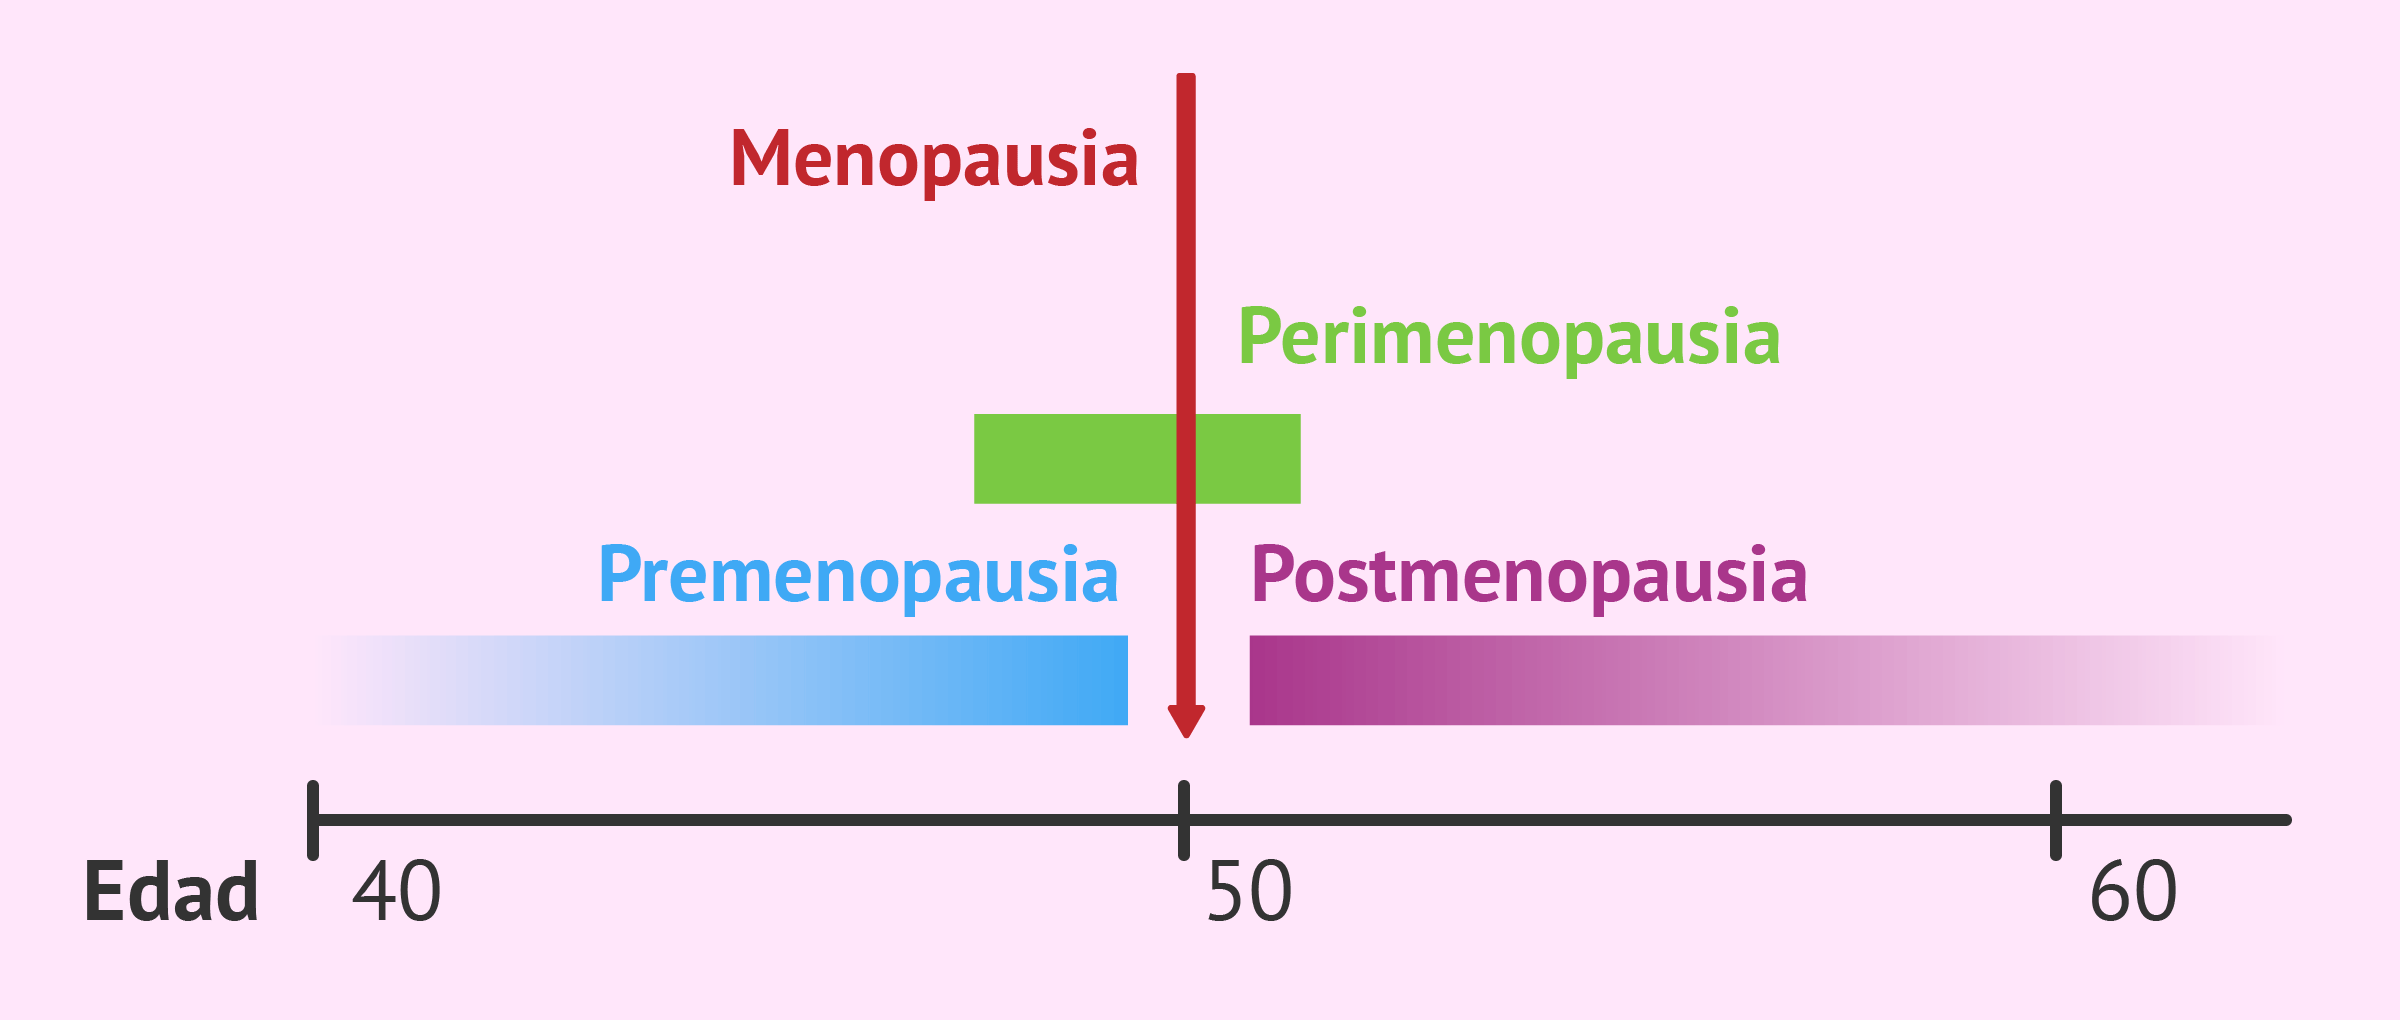
\includegraphics[width=1\linewidth]{IMAGENES/menopausia}\end{center}
			\\ \hline
			
			%------------------------------------------------------	
			Metastatic tumor indicator
			& El \textit{Indicador de tumor metastásico} se clasifica de forma nominal en dos categorías: La primera categoría corresponde al estado \textit{No}, en donde se encuentran 807 pacientes en los que el cáncer no se extendió desde el tumor primario a órganos o ganglios linfáticos distantes. La segunda categoría corresponde al estado \textit{Si}, en donde se encuentran 11 pacientes en los que el cáncer se extendió desde el tumor primario a órganos o ganglios linfáticos distantes.
			
			& \begin{center}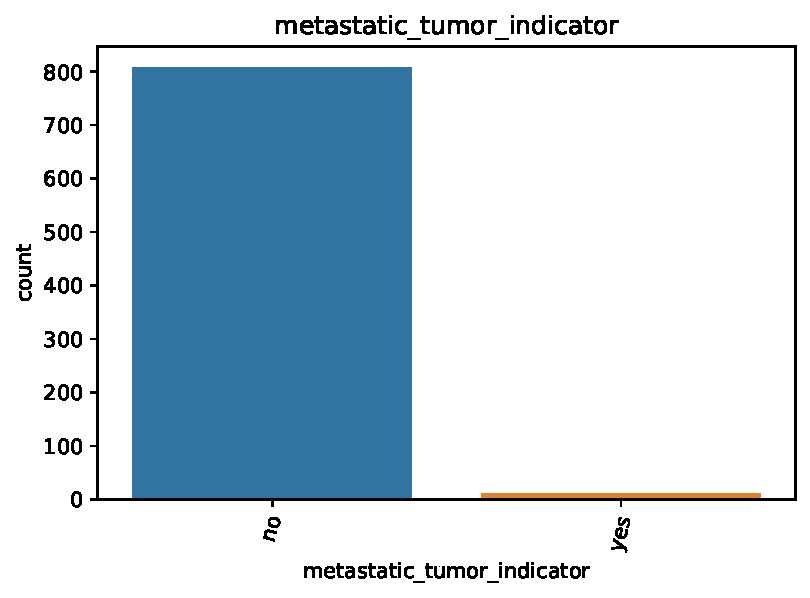
\includegraphics[width=1\linewidth]{NOTEBOOK/IMAGENES_DESCRIPTIVAS/33_metastatic_tumor_indicator}\end{center}
			\\ \hline
			
			%------------------------------------------------------	
			First Pathologic Diagnosis Biospecimen Acquisition Method Type
			& El \textit{tipo de método para adquisición de muestras biológicas} realizado en el primer diagnostico patológico, se visualiza en orden descendente de la siguiente manera: En primer lugar, la intervención quirúrgica de \textit{Biopsia con aguja gruesa (CNB)} se realizo a 495 pacientes en los cuales el medico utilizo una aguja hueca unida a una herramienta con resorte para extraer pedazos de tejido mamario de un área sospechosa. En segundo lugar, la intervención quirúrgica de \textit{resección tumoral} se realizo a 495 pacientes a los cuales se les extirpo todo el tumor o la mayor cantidad posible del mismo. En tercer lugar, la la intervención quirúrgica de \textit{Aspiración con aguja fina (FNA)} se realizo a 83 pacientes en los cuales el medico utilizo una aguja hueca muy delgada unida a una jeringa para extraer una pequeña cantidad de tejido mamario o líquido de un área sospechosa. En cuarto lugar, 59 pacientes utilizaron \textit{otros} tipos de métodos para adquisición de muestras biológicas. 
			& \begin{center}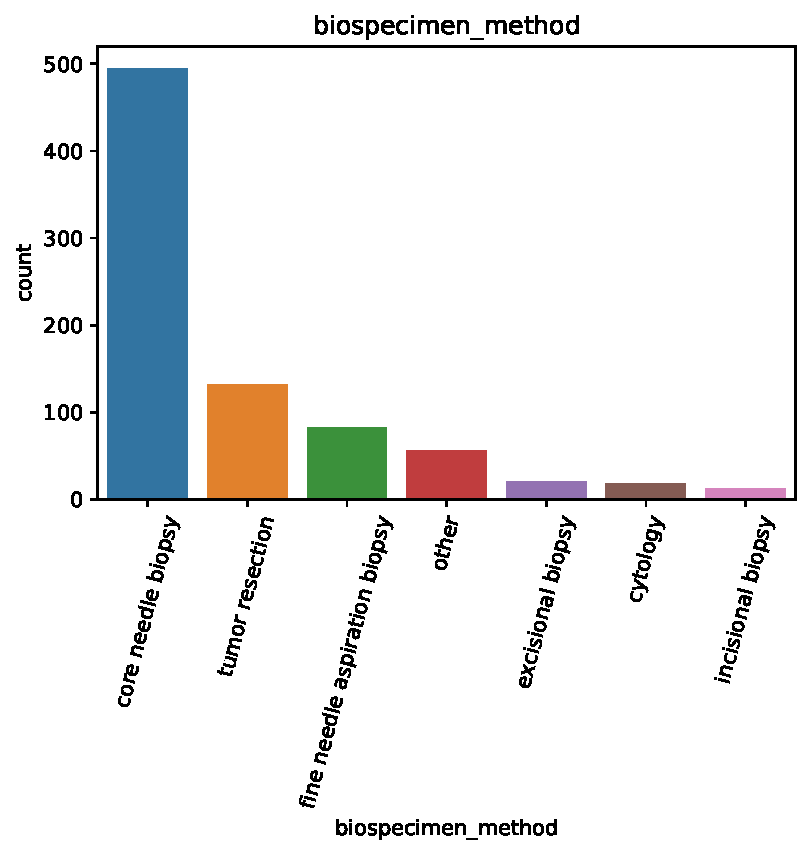
\includegraphics[width=1\linewidth]{NOTEBOOK/IMAGENES_DESCRIPTIVAS/34_biospecimen_method}\end{center}
			\\ \hline
		\end{tabular}
	\end{threeparttable}
\end{table*}

\begin{table*}[!htb]
	\footnotesize
	\begin{threeparttable}
		\begin{tabular}{p{2.5cm} p{7cm} p{6.5cm}} \toprule
			%--Continuacion,First Pathologic Diagnosis Biospecimen Acquisition Method Type
			&  En quinto lugar, la intervención quirúrgica \textit{Biopsia por escisión} se realizo a 21 pacientes a los cuales se les extirpo una masa completa o área sospechosa.En sexto lugar, la \textit{Citología} se realizó a 18 pacientes en donde se registró la simetría, el tamaño y la forma de la mama, así como cualquier evidencia de edema (piel de naranja), retracción del pezón o de la piel y eritema. En séptimo lugar, la intervención quirúrgica \textit{Biopsia por incisión} se realizo a 21 pacientes a los cuales se les extirpo una masa completa o área sospechosa
			& 
			\\ \hline
			
			%------------------------------------------------------	
			Micromet detection by ihc 
			& La \textit{Detección de micrometástasis según el método de tinción inmunohistoquímica(IHC) de citoqueratina(CK)} se clasifica de forma nominal en dos categorías: La primera categoría corresponde al estado \textit{No} en donde se encuentran 643 pacientes en los que se detecto la presencia de micrometástasis. La segunda categoría corresponde al estado \textit{Si} en donde se encuentran 175  pacientes en los que se detecto la presencia de micrometástasis conformada por grupos de células cancerosas que tienen entre 0,2 milímetros y 2 milímetros  utilizando el método inmunohistoquímica (IHC) de citoqueratina(CK).
			& \begin{center}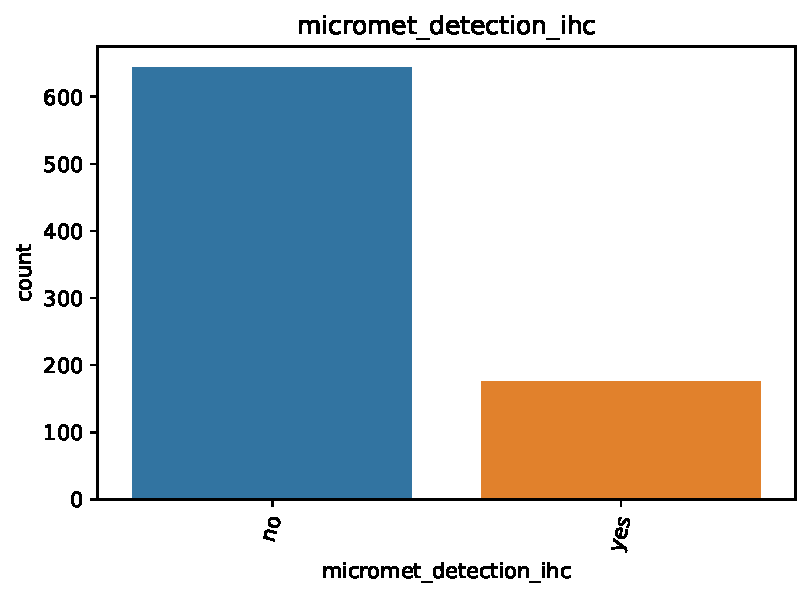
\includegraphics[width=1\linewidth]{NOTEBOOK/IMAGENES_DESCRIPTIVAS/35_micromet_detection_ihc}\end{center}
			\\ \hline
			
			%------------------------------------------------------	
			Mutation Count
			& El \textit{recuento de mutaciones} en el ADN el cual ocasiona que una célula sana  crezca y se divida con mayor rapidez, tiene  una tendencia central aproximada de 36 mutaciones, en donde el número mínimo de mutaciones es 1 y el número máximo de mutaciones es 3860.
			& \begin{center}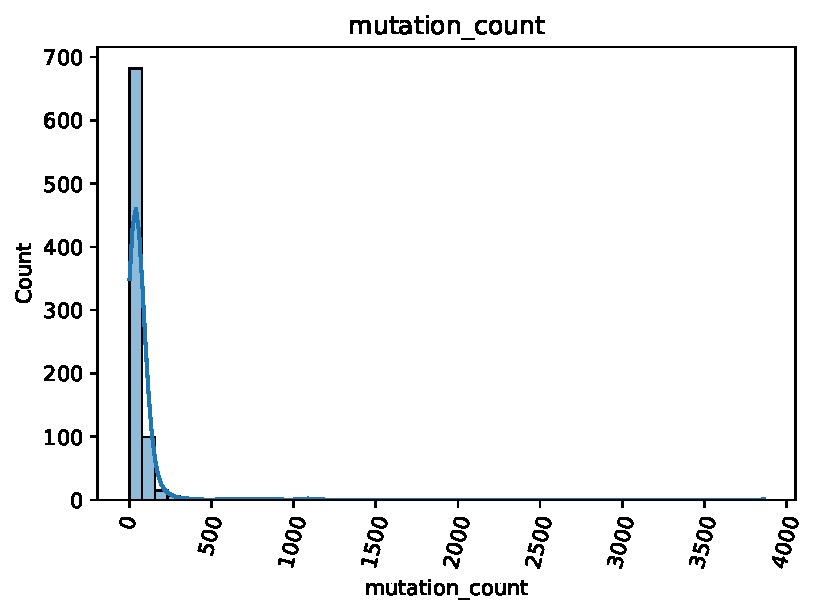
\includegraphics[width=1\linewidth]{NOTEBOOK/IMAGENES_DESCRIPTIVAS/36_mutation_count}\end{center}
			\\ \hline
			
			%------------------------------------------------------	
			Oct embedded
			& El uso del \textit{compuesto de temperatura de corte óptimo(OCT)} se clasifica de forma nominal en dos categorías: La primera categoría corresponde al estado \textit{Verdadero}, en donde se encuentran 481 pacientes, en los cuales la adquisición de muestras se realizo mediante el proceso OCT para generar secciones de tejidos en un portaobjetos para posteriormente generar el análisis histopatológico. La segunda categoría corresponde al estado \textit{Falso}, en donde se encuentran 337 pacientes, en los cuales la adquisición de muestras no se utilizo el proceso OCT.
			& \begin{center}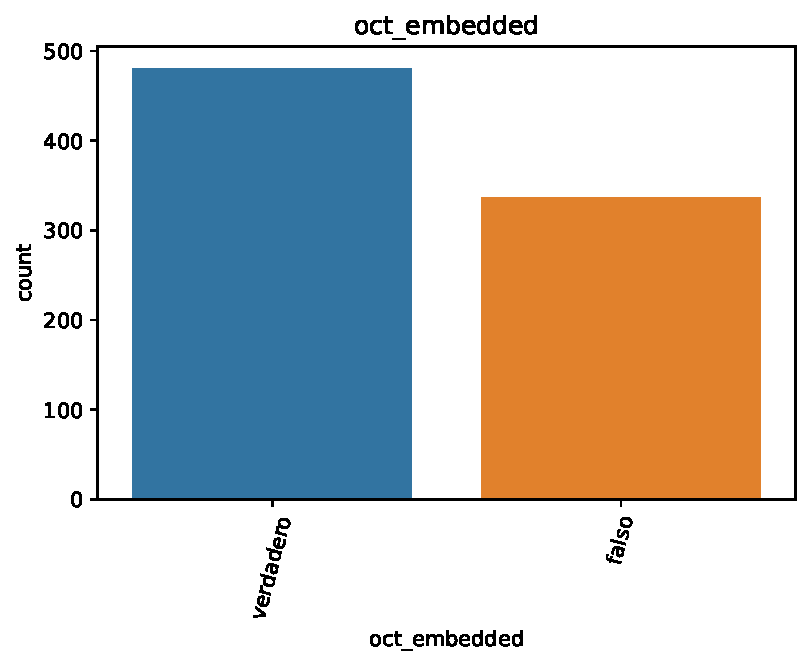
\includegraphics[width=1\linewidth]{NOTEBOOK/IMAGENES_DESCRIPTIVAS/37_oct_embedded}\end{center}
			\\ \hline
		\end{tabular}
	\end{threeparttable}
\end{table*}






